\documentclass[a4paper,12pt]{article}
\setcounter{secnumdepth}{2}
\newcommand{\code}[1]{{\footnotesize{{\tt #1}}}}
\usepackage{natbib}
\usepackage{color}
\usepackage{graphicx}
\usepackage{listings}
\lstset{
basicstyle=\small\ttfamily,
columns=flexible,
breaklines=true
}
\addtolength{\textwidth}{2cm} % a = -2b, where this is a and below is b
\addtolength{\hoffset}{-1cm}
\addtolength{\textheight}{2cm} % c = -d, where this is c and d is below
\addtolength{\voffset}{-2cm}
\begin{document}
\title{BayesNetty: Bayesian Network Software for Genetic Analyses}
\date{}
\author{Richard Howey\\Population Health Sciences Institute, Newcastle University, UK}
\maketitle
\newpage
\tableofcontents
\newpage
\section{Introduction}
\label{introduction}

BayesNetty is a C++ program written to perform Bayesian network analyses using genetic and phenotypic data. 

BayesNetty is copyright, 2015-present Richard Howey, GNU General Public License, version 3. 

/newline /newline

The {\bf recommended use} of BayesNetty is to calculate the average network as described in  section \ref{average-network}, possibly additionally using imputation to fill in missing data as descibed in  section \ref{impute-data}. However, for new users we reccomend you work your way through all sections in numerical order, in order to understand the functionality of the program. 

%================== End of section "introduction"==================

\section{Installation}
\label{installation}

Download an executable file from the download$\:$page for your system and off you go, or do the following: 
\begin{enumerate}

\item Download the code from the download page. 
\item Compile it by typing something like the following: \vspace{0.35cm} \begin{lstlisting}
g++ -m64 -O3 *.cpp -o bayesnetty 
\end{lstlisting} \vspace{0.35cm}
\item Start using BayesNetty!\end{enumerate}

%================== End of section "installation"==================

\section{Using BayesNetty}
\label{using}

BayesNetty is executed as follows: 
\vspace{0.35cm} \begin{lstlisting}

 ./bayesnetty paras.txt

\end{lstlisting} \vspace{0.35cm}
where \code{paras.txt} is a parameter file as described in the following sections. 
\subsection{Basic Options}
\label{basic-options}

The basic options for BayesNetty are as follows (typing \code{./bayesnetty} with no options will output the available options): 

{\begin{center}\begin{tabular}{lll}
Option  & Description  & Default\\
\hline
-log file.log  & log file of screen output  & bayesnetty.log\\
-so  & suppress output to screen  & \\
-seed number  & random number generator seed  & set by execution time\\
\end{tabular}\end{center}}
\subsubsection{Random Seed}
\label{random-seed}
The random seed option \code{-seed} may be used to ensure exactly the same output for testing and reproducibility purposes. If you do this it is important to use the same number of processes if also using the parallel version of BayesNetty.
%====== End of subsubsection "random-seed"======


%============ End of subsection "basic-options"============

\subsection{Parameter file}
\label{parameterfile}

There are many different things that BayesNetty can do, each of these different things is referred to as a ``task''. The parameter file defines which tasks BayesNetty will perform and the order in which they are executed. With the exception of the basic options in  section \ref{basic-options}, all options in the parameter file define tasks. For example, a task to input some continuous data may be given as follows: 
\vspace{0.35cm} \begin{lstlisting}

-input-data
-input-data-name myGreatData
-input-data-file example-cts.dat
-input-data-cts
-input-data-ids 1

\end{lstlisting} \vspace{0.35cm}
There are a few basic rules for parameter files: 
\begin{enumerate}

\item Each option must be written on a separate line. 
\item Each line that does not start with a dash, ``-'', will be ignored, thus allowing comments to be written. 
\item The task must first be declared and then followed by any options for the task. 
\item An option for a task is always written by first writing the name of the task. For example, the task option to give the name of an input data file is given by \code{-input-data-file}, which begins with \code{-input-data}, the name of the task to input data. 
\item A task, \code{XXX}, may always be given a task name with the option \code{XXX-name}. The task may then be referenced by other tasks (if permitted). This may be useful if there is more than one network. 
\item Tasks are executed in order, so any tasks that depend on other tasks must be ordered accordingly. 
\item Any tasks that require a network will be default use the previously defined network. Therefore, if there is only one network it is not necessary to name or reference it. By default tasks are name ``Task-n'', where n is the number of the task.\end{enumerate}

The following is an extract from an example parameter file where a network is referenced by a task to calculate the network score: 
\vspace{0.35cm} \begin{lstlisting}


...

# This is my comment
-input-network
-input-network-name myNetwork
-input-network-file network-model.dat

-calc-network-score
-calc-network-score-network-name myNetwork

\end{lstlisting} \vspace{0.35cm}
The parameter file could be thought of as in an \code{R} programming style, such that the above would look as follows: 
\vspace{0.35cm} \begin{lstlisting}


...

# This is my comment
myNetwork<-input.network(file = "network-model.dat")

calc.network.score(network.name = myNetwork)

\end{lstlisting} \vspace{0.35cm}
However, as BayesNetty is not an \code{R} package (or a programming language), the parameter file uses an unambiguous, longhand, and easy to parse style of syntax. 

The options for all the different tasks may be found in the different task sections of the documentation. 

%============ End of subsection "parameterfile"============

\subsection{Simple Example}
\label{simple-example}

Example data and parameter files can be found in the file example.zip. The example parameter file, \code{paras-example.txt}, can be used to perform a simple analysis by typing 
\vspace{0.35cm} \begin{lstlisting}

 ./bayesnetty paras-example.txt

\end{lstlisting} \vspace{0.35cm}
The following shows the \code{paras-example.txt} file 
\vspace{0.35cm} \begin{lstlisting}

#input continuous data
-input-data
-input-data-file example-cts.dat
-input-data-cts

#input discrete data
-input-data
-input-data-file example-discrete.dat
-input-data-discrete

#input SNP data as discrete data
-input-data
-input-data-file example.bed
-input-data-discrete-snp

#search network models
-search-models
-search-models-file search-example.dat

\end{lstlisting} \vspace{0.35cm}
The parameter file instructs BayesNetty to perform 4 tasks: (i) load continuous data from file \code{example-cts.dat}; (ii) load discrete data from file \code{example-discrete.dat}; (iii) load SNP data to be treated as discrete data from file \code{example.bed}; and finally (iv) search the network models. The screen output, which is also saved to a log file, will look something as follows: 
\vspace{0.35cm} \begin{lstlisting}

BayesNetty: Bayesian Network software, v1.00
--------------------------------------------------
Copyright 2015-present Richard Howey, GNU General Public License, v3
Institute of Genetic Medicine, Newcastle University

Random seed: 1551700145
--------------------------------------------------
Task name: Task-1
Loading data
Continuous data file: example-cts.dat
Number of ID columns: 2
Including (all) 2 variables in analysis
Each variable has 1500 data entries
Missing value: not set
--------------------------------------------------
--------------------------------------------------
Task name: Task-2
Loading data
Discrete data file: example-discrete.dat
Number of ID columns: 2
Including the 1 and only variable in analysis
Each variable has 1500 data entries
Missing value: NA
--------------------------------------------------
--------------------------------------------------
Task name: Task-3
Loading data
SNP binary data file: example.bed
SNP data treated as discrete data
Total number of SNPs: 2
Total number of subjects: 1500
Number of ID columns: 2
Including (all) 2 variables in analysis
Each variable has 1500 data entries
--------------------------------------------------
--------------------------------------------------
Task name: Task-4
Searching network models
--------------------------------------------------
Loading defaultNetwork network
Network type: bnlearn
Network score type: BIC
Total number of nodes: 5 (Discrete: 3 | Factor: 0 | Continuous: 2)
Total number of edges: 0
Network Structure: [express][pheno][mood][rs1][rs2]
Total data at each node: 1495
Missing data at each node: 5
--------------------------------------------------
Network: defaultNetwork
Search: Greedy
Random restarts: 0
Random jitter restarts: 0
Network Structure: [mood][rs1][rs2][express|rs1:rs2][pheno|express:mood]
Network score type: BIC
Network score = -8213.45
Network search output to file: search-example.dat
--------------------------------------------------

Run time: less than one second

\end{lstlisting} \vspace{0.35cm}
%============ End of subsection "simple-example"============

\subsection{Command-line Options}
\label{command-line}

It is also possible to add options on the command line to modify or add to the options in the parameter file. For example 
\vspace{0.35cm} \begin{lstlisting}

./bayesnetty paras-example.txt -seed 1 -log seed-1-results.log

\end{lstlisting} \vspace{0.35cm}
%============ End of subsection "command-line"============


%================== End of section "using"==================

\section{Parallel BayesNetty}
\label{parallel}

It is possible to run BayesNetty using Open MPI (\citet{openmpi}), which is an open source Message Passing Interface (MPI) (\citet{mpi}) implementation designed for parallel programming. 

The parallel version of Bayesnetty speeds up the search through network space for the best network by simultaneously evaluating different networks. This is particularly useful for large networks and any type of analysis that depends on network searches, such as network averaging and imputing data. 

A much faster way to calculate an average network in parallel is given in  section \ref{average-network-parallel}. 

A much faster way to impute network data in parallel is given in  section \ref{impute-parallel-example}. 

After installing Open MPI on your system if it is not already installed, see \citet{openmpi}, a parallel version of BayesNetty needs to be compiled. This can be done by firstly uncommenting a few lines in the \code{main.h} file. So that the following: 
\vspace{0.35cm} \begin{lstlisting}

// Comment out if not using Open MPI for parallel processing
//#ifndef USING_OPEN_MPI
//#define USING_OPEN_MPI
//#endif //OPEN_MPI

\end{lstlisting} \vspace{0.35cm}
becomes 
\vspace{0.35cm} \begin{lstlisting}

// Comment out if not using Open MPI for parallel processing
#ifndef USING_OPEN_MPI
#define USING_OPEN_MPI
#endif //OPEN_MPI

\end{lstlisting} \vspace{0.35cm}
then compile the parallel code as follows: 
\vspace{0.35cm} \begin{lstlisting}

mpicxx -O3 -o pbayesnetty *.cpp

\end{lstlisting} \vspace{0.35cm}
The code can then be ran using how many processes that you wish, for example to run with 12 processes use 
\vspace{0.35cm} \begin{lstlisting}

mpirun -n 12 ./pbayesnetty paras-example.txt

\end{lstlisting} \vspace{0.35cm}
For such a trivial example the code will not run any quicker, and in fact for very small networks one may find that analyses take longer. There is some overhead in using the MPI libraries, so if trivial networks are used there may be no speed up. 

Even for large networks the optimal number of processes to perform the analysis as quick as possible may not be as many processes as you can use. As there is an overhead for processes the best amount to use may be a lot, but not too many... The best amount will vary depending on the analysis, the data and the computing system that you are using, so some trial and error may be needed. 

The output will show the number of processes as well as the random seed. If you wish to reproduce exactly the same results both of these need to be set to the same value. The seed is set with the \code{-seed} option. 
\vspace{0.35cm} \begin{lstlisting}

BayesNetty: Bayesian Network software, v1.00
--------------------------------------------------
Copyright 2015-present Richard Howey, GNU General Public License, v3
Institute of Genetic Medicine, Newcastle University

Number of processes: 12
Random seed: 1541430503
--------------------------------------------------
Task name: Task-1
Loading data
Continuous data file: example-cts.dat
Number of ID columns: 2
Including (all) 2 variables in analysis
Each variable has 1500 data entries
Missing value: not set
--------------------------------------------------
--------------------------------------------------

...


\end{lstlisting} \vspace{0.35cm}\subsection{Compilation Scripts}
\label{compile-parallel-code}

Scripts to compile Bayesnetty as either parallel or non-parallel while automatically uncommenting or commenting the code as appropriate are given below. 

Script to compile code in parallel: 
\vspace{0.35cm} \begin{lstlisting}

sed -i s://#ifndef\ USING_OPEN_MPI:#ifndef\ USING_OPEN_MPI:g main.h
sed -i s://#define\ USING_OPEN_MPI:#define\ USING_OPEN_MPI:g main.h
sed -i s://#endif\ //:#endif\ //:g main.h

mpicxx -O3 -o pbayesnetty *.cpp

\end{lstlisting} \vspace{0.35cm}
Script to compile code in non-parallel: 
\vspace{0.35cm} \begin{lstlisting}

sed -i s://#ifndef\ USING_OPEN_MPI:#ifndef\ USING_OPEN_MPI:g main.h
sed -i s://#define\ USING_OPEN_MPI:#define\ USING_OPEN_MPI:g main.h
sed -i s://#endif\ //:#endif\ //:g main.h

sed -i s:#ifndef\ USING_OPEN_MPI://#ifndef\ USING_OPEN_MPI:g main.h
sed -i s:#define\ USING_OPEN_MPI://#define\ USING_OPEN_MPI:g main.h
sed -i s:#endif\ //://#endif\ //:g main.h

g++ -O3 *.cpp -o bayesnetty

\end{lstlisting} \vspace{0.35cm}
%============ End of subsection "compile-parallel-code"============


%================== End of section "parallel"==================

\section{Input data}
\label{input-data}

All data must be input using the \code{-input-data} task. 
\subsection{Options}
\label{input-data-options}

The options are as follows: 

{\begin{center}\resizebox{16cm}{!}{\begin{tabular}{lp{9cm}l}
Option  & Description  & Default\\
\hline
-input-data  & do a task to input data  & \\
-input-data-name name  & label the task with a name  & Task-n\\
-input-data-file data.dat  & the file containing the data for each network node  & \\
-input-data-include-file nodes.dat  & a list of nodes/variables from the data file to be included in the network. Only the nodes in this list will be used in any analysis.  & \\
-input-data-exclude-file nodes.dat  & a list of nodes/variables to be excluded from the network  & \\
-input-data-cts  & set the data file as containing continuous data  & \\
-input-data-cts-snp  & set the .bed data file as containing SNP data to be treated as continuous data (0, 1, 2) in the network  & \\
-input-data-cts-snp2  & set the data file as containing continuous SNP data (taking any continuous values)  & \\
-input-data-cts-missing-value x  & set the value of missing data for continuous data to x  & \\
-input-data-discrete  & set the data file as containing discrete data  & \\
-input-data-discrete-snp  & set the .bed data file as containing SNP data to be treated as discrete data in the network  & \\
-input-data-discrete-snp2  & set the data file as containing discrete SNP data (taking any number of discrete values)  & \\
-input-data-discrete-missing-value x  & set the value of missing data for discrete data to x  & NA\\
-input-data-factor  & set the data file as containing discrete data encoded using factor variables  & \\
-input-data-factor-snp  & set the .bed file as containing SNP data to be treated as discrete factor data in the network  & \\
-input-data-factor-snp2  & set the data file as containing discrete factor SNP data (taking any number of discrete values)  & \\
-input-data-factor-missing-value x  & set the value of missing data for discrete factor data to x  & NA\\
-input-data-ids n  & the number of ID columns in each data file  & 2\\
-input-data-csv  & set the data file as a comma separated file, .csv  & \\
\end{tabular}}\end{center}}

%============ End of subsection "input-data-options"============

\subsection{Discrete data}
\label{input-data-discrete}

Discrete data is automatically constrained to have no parent nodes that are continuous. 

Discrete data is input by using the \code{-input-data} task, setting the data file and setting the data file to discrete. For example, the following 
\vspace{0.35cm} \begin{lstlisting}

-input-data
-input-data-file example-discrete.dat
-input-data-discrete

\end{lstlisting} \vspace{0.35cm}
could be used and the output would be something as follows: 
\vspace{0.35cm} \begin{lstlisting}

BayesNetty: Bayesian Network software, v1.00
--------------------------------------------------
Copyright 2015-present Richard Howey, GNU General Public License, v3
Institute of Genetic Medicine, Newcastle University

Random seed: 1551695824
--------------------------------------------------
Task name: Task-1
Loading data
Discrete data file: example-discrete.dat
Number of ID columns: 2
Including the 1 and only variable in analysis
Each variable has 1500 data entries
Missing value: NA
--------------------------------------------------

Run time: less than one second

\end{lstlisting} \vspace{0.35cm}
This parameter file can be found \code{paras-input-discrete.txt} in the examples, example.zip. 

%============ End of subsection "input-data-discrete"============

\subsection{Continuous data}
\label{input-data-cts}

Continuous data is input by using the \code{-input-data} task, setting the data file and setting the data file to continuous. For example, the following 
\vspace{0.35cm} \begin{lstlisting}

-input-data
-input-data-file example-cts.dat
-input-data-cts

\end{lstlisting} \vspace{0.35cm}
could be used and the output would be something as follows: 
\vspace{0.35cm} \begin{lstlisting}

BayesNetty: Bayesian Network software, v1.00
--------------------------------------------------
Copyright 2015-present Richard Howey, GNU General Public License, v3
Institute of Genetic Medicine, Newcastle University

Random seed: 1551695897
--------------------------------------------------
Task name: Task-1
Loading data
Continuous data file: example-cts.dat
Number of ID columns: 2
Including (all) 2 variables in analysis
Each variable has 1500 data entries
Missing value: not set
--------------------------------------------------

Run time: less than one second

\end{lstlisting} \vspace{0.35cm}
This parameter file can be found \code{paras-input-cts.txt} in the examples, example.zip. 

%============ End of subsection "input-data-cts"============

\subsection{Factor data}
\label{input-data-factor}

Another way of handling discrete data is with the use of {\it factors}. Indicator variables are created, one for each different discrete category minus one. These are treated as continuous explanatory variables in the linear regressions when they are parent nodes. A restriction of using discrete data with factors is that they cannot be child nodes of other nodes. Input by using the \code{-input-data} task, setting the data file and setting the data file to factor. For example, the following 
\vspace{0.35cm} \begin{lstlisting}

-input-data
-input-data-file example-discrete.dat
-input-data-factor

\end{lstlisting} \vspace{0.35cm}
could be used and the output would be something as follows: 
\vspace{0.35cm} \begin{lstlisting}

BayesNetty: Bayesian Network software, v1.00
--------------------------------------------------
Copyright 2015-present Richard Howey, GNU General Public License, v3
Institute of Genetic Medicine, Newcastle University

Random seed: 1551695930
--------------------------------------------------
Task name: Task-1
Loading data
Discrete data file: example-discrete.dat
Data treated as factors
Number of ID columns: 2
Including the 1 and only variable in analysis
Each variable has 1500 data entries
Missing value: NA
--------------------------------------------------

Run time: less than one second

\end{lstlisting} \vspace{0.35cm}
This parameter file can be found \code{paras-input-factor.txt} in the examples, example.zip. 

%============ End of subsection "input-data-factor"============

\subsection{SNP data}
\label{input-data-snp}

SNP data is automatically constrained to have no parent nodes. 

SNP data may be input as a binaryPLINK format pedigree file, a \code{.bed} file, see \citet{purcell:etal:07}. This requires that the corresponding \code{.bim} and \code{.fam}, files are also available. A text PLINK pedigree file, \code{.ped}, with corresponding map file, \code{.map}, may be used to create a binary file using PLINK as follows: \vspace{0.35cm} \begin{lstlisting}

plink --noweb --file mydata --make-bed --out myfile

\end{lstlisting} \vspace{0.35cm}

This will create the binary pedigree file, \code{myfile.bed}, map file, \code{myfile.bim}, and family file, \code{myfile.fam} required. 

The SNP data is input by using the \code{-input-data} task, setting the PLINK binary file and setting the data file to a SNP file in discrete mode or continuous mode. For example, in discrete mode, the following 
\vspace{0.35cm} \begin{lstlisting}

-input-data
-input-data-file example.bed
-input-data-discrete-snp

\end{lstlisting} \vspace{0.35cm}
could be used and the output would be something as follows: 
\vspace{0.35cm} \begin{lstlisting}

BayesNetty: Bayesian Network software, v1.00
--------------------------------------------------
Copyright 2015-present Richard Howey, GNU General Public License, v3
Institute of Genetic Medicine, Newcastle University

Random seed: 1551695984
--------------------------------------------------
Task name: Task-1
Loading data
SNP binary data file: example.bed
SNP data treated as discrete data
Total number of SNPs: 2
Total number of subjects: 1500
Number of ID columns: 2
Including (all) 2 variables in analysis
Each variable has 1500 data entries
--------------------------------------------------

Run time: less than one second

\end{lstlisting} \vspace{0.35cm}
This parameter file can be found \code{paras-input-snp.txt} in the examples, example.zip. 

%============ End of subsection "input-data-snp"============

\subsection{Missing data}
\label{input-data-missing}

Missing data is determined by any data matching the given missing value as defined by \code{-input-data-discrete-missing-value} and \code{-input-data-cts-missing-value} when inputting discrete and continuous data respectively (or \code{-input-data-factor-missing-value} when inputting factor data). When continuous data has an invalid entry this will also be set to missing, for example a value of ``NaN'' will be set to missing since a numerical value is required. Missing data for SNP data is given as defined by the PLINK binarypedigree format. When there is missing data for a node for a certain individual then data for this certain individual is considered as missing for {\it every} node in the network. Therefore the amount of missing data depends on which nodes are in the network. 

Consider a network with 2 continuous nodes, with structure as given by network file \code{example-network-missing1.dat} and input using parameter file \code{paras-input-missing1.txt} as given in example.zip,then the output will be will look something as follows: 
\vspace{0.35cm} \begin{lstlisting}

BayesNetty: Bayesian Network software, v1.00
--------------------------------------------------
Copyright 2015-present Richard Howey, GNU General Public License, v3
Institute of Genetic Medicine, Newcastle University

Random seed: 1551694585
--------------------------------------------------
Task name: Task-1
Loading data
Continuous data file: example-cts.dat
Number of ID columns: 2
Including (all) 2 variables in analysis
Each variable has 1500 data entries
Missing value: not set
--------------------------------------------------
--------------------------------------------------
Task name: myNetwork
Loading network
Network file: example-network-missing1.dat
Network type: bnlearn
Network score type: BIC
Total number of nodes: 2 (Discrete: 0 | Factor: 0 | Continuous: 2)
Total number of edges: 1
Network Structure: [express][pheno|express]
Total data at each node: 1500
Missing data at each node: 0
--------------------------------------------------

Run time: less than one second

\end{lstlisting} \vspace{0.35cm}
As indicated in the network details there is no missing data. However, if the SNP node, \code{rs1}, is added (network file \code{example-network-missing2.dat}) then the following is given: 
\vspace{0.35cm} \begin{lstlisting}

BayesNetty: Bayesian Network software, v1.00
--------------------------------------------------
Copyright 2015-present Richard Howey, GNU General Public License, v3
Institute of Genetic Medicine, Newcastle University

Random seed: 1551696539
--------------------------------------------------
Task name: Task-1
Loading data
SNP binary data file: example.bed
SNP data treated as discrete data
Total number of SNPs: 2
Total number of subjects: 1500
Number of ID columns: 2
Including (all) 2 variables in analysis
Each variable has 1500 data entries
--------------------------------------------------
--------------------------------------------------
Task name: Task-2
Loading data
Continuous data file: example-cts.dat
Number of ID columns: 2
Including (all) 2 variables in analysis
Each variable has 1500 data entries
Missing value: not set
--------------------------------------------------
--------------------------------------------------
Task name: myNetwork
Loading network
Network file: example-network-missing2.dat
Network type: bnlearn
Network score type: BIC
Total number of nodes: 3 (Discrete: 1 | Factor: 0 | Continuous: 2)
Total number of edges: 2
Network Structure: [rs1][express|rs1][pheno|express]
Total data at each node: 1497
Missing data at each node: 3
--------------------------------------------------

Run time: less than one second

\end{lstlisting} \vspace{0.35cm}
This example is given in network file \code{example-network-missing2.dat} and parameter file \code{paras-input-missing2.txt}. The amount of missing data for the network is now 3, indicating that 3 individuals have missing SNP data for \code{rs1}. Adding in another SNP node, \code{rs2} (network file \code{example-network-missing3.dat}), results in the following: 
\vspace{0.35cm} \begin{lstlisting}

BayesNetty: Bayesian Network software, v1.00
--------------------------------------------------
Copyright 2015-present Richard Howey, GNU General Public License, v3
Institute of Genetic Medicine, Newcastle University

Random seed: 1551696644
--------------------------------------------------
Task name: Task-1
Loading data
SNP binary data file: example.bed
SNP data treated as discrete data
Total number of SNPs: 2
Total number of subjects: 1500
Number of ID columns: 2
Including (all) 2 variables in analysis
Each variable has 1500 data entries
--------------------------------------------------
--------------------------------------------------
Task name: Task-2
Loading data
Continuous data file: example-cts.dat
Number of ID columns: 2
Including (all) 2 variables in analysis
Each variable has 1500 data entries
Missing value: not set
--------------------------------------------------
--------------------------------------------------
Task name: myNetwork
Loading network
Network file: example-network-missing3.dat
Network type: bnlearn
Network score type: BIC
Total number of nodes: 4 (Discrete: 2 | Factor: 0 | Continuous: 2)
Total number of edges: 3
Network Structure: [rs1][rs2][express|rs1:rs2][pheno|express]
Total data at each node: 1495
Missing data at each node: 5
--------------------------------------------------

Run time: less than one second

\end{lstlisting} \vspace{0.35cm}
Similarly, this example is given in network file \code{example-network-missing3.dat} and parameter file \code{paras-input-missing3.txt}. Here we see that the amount of missing data in the network has increased due to missing data for SNP node \code{rs2}. This node also has missing data for 3 individuals, with the result that the total amount of missing data for each node is 5. 

%============ End of subsection "input-data-missing"============

\subsection{Data IDs}
\label{input-data-ids}

By default the first two columns of a data file should be IDs and match those in any other data files, and be in the same order (although the ID names in the header do not need to match). The number of ID columns can be changed using the \code{-input-data-ids} option, and may be set to zero. If the data contains SNP data in a PLINK binary pedigree file, \code{.bed}, then the number of ID columns must be set to 2. If the data is a binary pedigree file, \code{file.bed}, then the family and individual IDs in the file \code{file.fam} must match the IDs in any other data files, and all SNPs may be used as network nodes. The IDs in different files are checked to be the same including the order, if not BayesNetty will report an error. If there are zero IDs then the individuals are assumed to be in the same order in each file and are only checked to have the same number of individuals. 

%============ End of subsection "input-data-ids"============

\subsection{Example}
\label{input-data-example}

See the above sections for examples of inputting data. 

%============ End of subsection "input-data-example"============


%================== End of section "input-data"==================

\section{Input network}
\label{input-network}

A network may be specified using the \code{-input-network} task. The network may be used as a starting point for analyses, such as searches, or to perform an analysis on this network. Only nodes in input files will be used in the network so that a subset of the data may be specified. 

Any network {\bf constraints} must be set using the \code{-input-network} option. These constraints then belong to the network and will be used in any subsquent analysis, including searches, calculating average networks etc. 

If no network is specified then a network with no edges and a node for every data variable (as given by the input data) will be created and named ``defaultNetwork''. 
\subsection{Options}
\label{input-network-options}

The options are as follows: 

{\begin{center}\resizebox{16cm}{!}{\begin{tabular}{lp{9cm}l}
Option  & Description  & Default\\
\hline
-input-network  & do a task to input a network  & \\
-input-network-name name  & label the task and network with a name  & Task-n\\
-input-network-type t  & the type of Bayesian network, choose between bnlearn or deal  & bnlearn\\
-input-network-file network.dat  & input the network in a format where the nodes and then the edges are listed  & \\
-input-network-file2 network2.dat  & input the network in this style of format: \code{[a][b|a][c|a:b]}  & \\
-input-network-igraph-file-prefix mygraph  & input the network from igraph format files consisting of mygraph-nodes.dat and mygraph-edges.dat  & \\
-input-network-empty  & set the network to one with no edges and one node for every data variable. An input network file is not required if this option is used  & \\
-input-network-whitelist-file whitelist.dat  & a list of edges that must be included in any network  & \\
-input-network-blacklist-file blacklist.dat  & a list of edges that must {\it not} be included in any network  & \\
-input-network-blacklist-edge-type dataName1 dataName2  & edge types that may {\it not} be included in any network. The collection of nodes are given by the data input name, and so the data types must be given in different files  & \\
-input-network-no-parents-node nodeX  & nodeX must not have any parents (except for white edges)  & \\
-input-network-no-children-node nodeY  & nodeY must not have any children (except for white edges)  & \\
-input-network-prob-edge node1 node2 prob  & set the prior probability of edge direction of node1 to node2 as prob  & \\
-input-network-prob-edge-type nodeType1 nodeType2 prob  & set the prior probabilities of edge direction of nodeType1 to nodeType2 as prob  & \\
-input-network-imaginary-sample-size i  & for deal networks this sets the imaginary sample size  & 10\\
-input-network-score score  & for a bnlearn network choose between loglike, AIC or BIC  & BIC\\
\end{tabular}}\end{center}}

%============ End of subsection "input-network-options"============

\subsection{Black lists}
\label{input-network-black}

A black list can be given using the \code{-input-network-blacklist-file} option to define a list of edges that must not be included in any network. The text file should be formatted as follows: 
\vspace{0.35cm} \begin{lstlisting}

node1 node2
node2 node1
node1 node3

\end{lstlisting} \vspace{0.35cm}
such that the two nodes of each blacklisted edge are on one line. The nodes are ordered so the first line states that the edge node1 to node2 is not permitted. The next line states that the edge in the reverse direction is also not permitted. 

Any searches will ignore these blacklisted edges and attempting to use a network with a blacklisted edge will result in the edge being removed. 

Edges between different types of nodes may also be blacklisted. This can be done using the \code{-input-network-blacklist-edge-type} option. It can be used as follows: 
\vspace{0.35cm} \begin{lstlisting}

-input-data
-input-data-name horses
-input-data-file horses.dat
-input-data-cts

-input-data
-input-data-name whips
-input-data-file whips.dat
-input-data-cts

-input-network
-input-network-name race
-input-network-file model.dat
-input-network-blacklist-edge-type horses whips 

\end{lstlisting} \vspace{0.35cm}
Firstly the different node types must be loaded separately and given names using the \code{-input-data-name} option. Then, when initially loading a network, the \code{-input-network-blacklist-edge-type} can be used to forbid any edge from one data set to another data set (or the same data if desired). In the above example the network may not have any edge that goes from a horse to a whip, that is, a whip node may not have a horse node as a parent. In any search that is performed these edges will not be considered. 

%============ End of subsection "input-network-black"============

\subsection{White lists}
\label{input-network-white}

A white list can be given using the \code{-input-network-whitelist-file} option to define a list of edges that must be included in any network. The text file should be formatted as follows: 
\vspace{0.35cm} \begin{lstlisting}

node1 node3
node1 node2
node2 node1

\end{lstlisting} \vspace{0.35cm}
such that the two nodes of each whitelisted edge are on one line. The nodes are ordered so the first line states that the edge node1 to node3 must be included. If both directions are included between two nodes then the edge must be included but may be in any direction. 

If the whitelist and blacklist contradict one another then an error will be given. 

%============ End of subsection "input-network-white"============

\subsection{Soft Constraints}
\label{input-network-soft-con}

Soft constraints provide a way that the direction of an edge may be influenced but not with certainty, unlike blacklisted edges or whitelisted edges as described above. An example parameter file setting a soft constraint, such that the prior probability of variable \code{express} to variable \code{pheno} is believed to be 0.8 is shown below. 
\vspace{0.35cm} \begin{lstlisting}

#input continuous data
-input-data
-input-data-file example-cts.dat
-input-data-cts

#input discrete data
-input-data
-input-data-file example-discrete.dat
-input-data-discrete

#input SNP data as discrete data
-input-data
-input-data-file example.bed
-input-data-discrete-snp

#input the example network in format 1
-input-network
-input-network-name myNetwork
-input-network-file example-network-format1.dat
-input-network-prob-edge express pheno 0.8

#search network models with the soft constraint
-search-models

\end{lstlisting} \vspace{0.35cm}
This parameter file, \code{paras-soft-constraints.txt}, can be found in example.zip.

Any searches will use this prior probability. 

If you wish to blacklist or whitelist an edge you should use those options rather than setting the prior probability to 0 or 1 for the sake of computational efficiency. 

%============ End of subsection "input-network-soft-con"============

\subsection{Network formats}
\label{input-network-formats}

The network may be defined using one of 3 different formats. 
\subsubsection{Network file format 1}
\label{input-network-formats-format1}

The first format is given by using the \code{-input-network-file} option and the network text file should be formatted as follows: 
\vspace{0.35cm} \begin{lstlisting}

node1
node2
node3
node2 node1
node3 node1

\end{lstlisting} \vspace{0.35cm}
where the nodes are listed first followed by the directed edges. In the above example there are 3 nodes and 2 edges, which are node2 to node1 and node3 to node1. 

%====== End of subsubsection "input-network-formats-format1"======

\subsubsection{Network file format 2}
\label{input-network-formats-format2}

The second format is given by using the \code{-input-network-file2} option and the network text file should be formatted as follows: 
\vspace{0.35cm} \begin{lstlisting}

[node2][node3][node1|node2:node3]

\end{lstlisting} \vspace{0.35cm}
where the nodes are listed in order of dependency. The independent nodes node2 and node3 are list first followed by node1 which is a child node of both node2 and node3. This is the format that is typically output for searches and such like. 

%====== End of subsubsection "input-network-formats-format2"======

\subsubsection{Network file format 3}
\label{input-network-formats-format3}

The third format is given by using the \code{-input-network-igraph-file-prefix} option using the files that were output to draw the network in \code{R}, see  section \ref{igraph}. There will be one file for the nodes and one for the edges, for example \code{myNetwork-nodes.dat} and \code{myNetwork-edges.dat} respectively. The node file will look something as follows: 
\vspace{0.35cm} \begin{lstlisting}

id name type fileno
1 node1 c 1
2 node2 c 1
3 node3 c 1

\end{lstlisting} \vspace{0.35cm}
and the edges file will look like something as follows: 
\vspace{0.35cm} \begin{lstlisting}

from to chisq
2 1 6860.83
3 1 5709.51

\end{lstlisting} \vspace{0.35cm}
%====== End of subsubsection "input-network-formats-format3"======


%============ End of subsection "input-network-formats"============

\subsection{Example}
\label{input-network-example}

The following is an example parameter file to input a network. 
\vspace{0.35cm} \begin{lstlisting}

#input continuous data
-input-data
-input-data-file example-cts.dat
-input-data-cts

#input discrete data
-input-data
-input-data-file example-discrete.dat
-input-data-discrete

#input SNP data as discrete data
-input-data
-input-data-file example.bed
-input-data-discrete-snp

#input the example network in format 1
-input-network
-input-network-name myNetwork
-input-network-file example-network-format1.dat

\end{lstlisting} \vspace{0.35cm}
This parameter file, \code{paras-input-network.txt}, can be found in example.zipand can be used as follows: 
\vspace{0.35cm} \begin{lstlisting}

./bayesnetty paras-input-network.txt

\end{lstlisting} \vspace{0.35cm}
Which should produce output that looks like something as follows: 
\vspace{0.35cm} \begin{lstlisting}

BayesNetty: Bayesian Network software, v1.00
--------------------------------------------------
Copyright 2015-present Richard Howey, GNU General Public License, v3
Institute of Genetic Medicine, Newcastle University

Random seed: 1551697141
--------------------------------------------------
Task name: Task-1
Loading data
Continuous data file: example-cts.dat
Number of ID columns: 2
Including (all) 2 variables in analysis
Each variable has 1500 data entries
Missing value: not set
--------------------------------------------------
--------------------------------------------------
Task name: Task-2
Loading data
Discrete data file: example-discrete.dat
Number of ID columns: 2
Including the 1 and only variable in analysis
Each variable has 1500 data entries
Missing value: NA
--------------------------------------------------
--------------------------------------------------
Task name: Task-3
Loading data
SNP binary data file: example.bed
SNP data treated as discrete data
Total number of SNPs: 2
Total number of subjects: 1500
Number of ID columns: 2
Including (all) 2 variables in analysis
Each variable has 1500 data entries
--------------------------------------------------
--------------------------------------------------
Task name: myNetwork
Loading network
Network file: example-network-format1.dat
Network type: bnlearn
Network score type: BIC
Total number of nodes: 5 (Discrete: 3 | Factor: 0 | Continuous: 2)
Total number of edges: 4
Network Structure: [mood][rs1][rs2][pheno|rs1:rs2][express|pheno:mood]
Total data at each node: 1495
Missing data at each node: 5
--------------------------------------------------

Run time: 1 second

\end{lstlisting} \vspace{0.35cm}
The data is loaded and then the network is loaded. The network has been named ``myNetwork'', and basic information about the network is output. 

Similarly, the network may be input using format 2 and 3 as given in parameter files \code{paras-input-network2.txt} and \code{paras-input-network3.txt} respectively. 

%============ End of subsection "input-network-example"============


%================== End of section "input-network"==================

\section{bnlearn network}
\label{bnlearn}

The default and recommended Bayesian network in BayesNetty is given by the bnlearn algorithm. All future extensions are intended to be built upon this approach. For a given data set and network structure the likelihood can be calculated under specific distributional assumptions, namely that discrete nodes follow a multinomial distribution and continuous nodes a normal distribution, with distributional parameters determined by the values of the incoming parent nodes. The manner in which the likelihood is calculated can vary between Bayesian network algorithms. See \citet{bnlearn} and \citet{bnlearn2} for further details of bnlearn methodology and R package. 
\subsection{Network score}
\label{bnlearn-score}

The network score for a bnlearn network may be set to either the log likelihood, AIC or BIC using the \code{-input-network-score} option, see  section \ref{input-network-options}. 

{\bf NOTE:} The BIC network score is based on the definition used by bnlearn (see \citet{bnlearn}) such that BIC = log(L) - (d/2)log(n), where L is the likelihood of the network for the given data set, d is the number of parameters and n is the number of individuals. This is the original definition used by Swartz in 1978, see \citet{swartz:1978}, rather than subsequent definitions of BIC which are multplied by negative two (for example see \citet{wit:2012}). Therefore in BayesNetty the BIC will always be negative and higher values of the network score imply a better fit network. (Whichever definition of BIC that one considers, the closer the BIC is to zero the better the model fit.) 

The AIC network score in BayesNetty is defined similarly to the BIC such that AIC = log(L) - d, where L and d are defined as above. Therefore higher values of the negatively valued AIC (closer to zero) imply a better network fit to the given data set. 

Naturally if only the log likelihood is used then higher values imply a better network fit. 

%============ End of subsection "bnlearn-score"============


%================== End of section "bnlearn"==================

\section{deal network}
\label{deal}

The deal Bayesian network approach was developed by \citet{deal} as an approach to model mixed discrete/continuous networks. It calculates the likelihood differently to bnlearn. However we found several issues with the method, not least that it is no longer actively supported. Therefore, it is not recommended to use a deal network for network analyses and is included only for comparison purposes. 
\subsection{Imaginary sample size}
\label{imaginary-sample-size}

When analysis is performed with a deal network the imaginary sample size (ISS) must be set. The ISS reflects how much confidence we have in the (in)dependencies expressed in the assumed prior network. This can be set using the \code{-input-network-imaginary-sample-size} option, see  section \ref{input-network-options}. The results given by deal have been found to be very sensitive to the setting of this parameter and there is no obvious ``good'' default setting. 

The network score in a deal network is based upon the log likelihood and so higher values imply a better network fit to the given data set. 

%============ End of subsection "imaginary-sample-size"============


%================== End of section "deal"==================

\section{Calculate network score}
\label{calc-score}

The network score is used as a measure of how well the network model describes the data and is used to compare different models when searching through models. In BayesNetty the network score is based on the log likelihood and higher values imply a better model (see  section \ref{bnlearn-score} for further details). This is calculated assuming that discrete nodes follow a multinomial distribution and continuous nodes a normal distribution. BayesNetty considers the network score to be a property of the network and its method of calculation is set using the option \code{-input-network-score}, see  section \ref{input-network}. 
\subsection{Options}
\label{calc-score-options}

The options are as follows: 

{\begin{center}\resizebox{16cm}{!}{\begin{tabular}{lp{9cm}l}
Option  & Description  & Default\\
\hline
-calc-network-score  & do a task to calculate the score  & \\
-calc-network-score-name name  & label the task with a name  & Task-n\\
-calc-network-score-network-name network  & the name of the network to calculate the score of  & previous network (or the default model given by a node for each data variable and no edges if there is no previous network)\\
-calc-network-score-file file  & write the score to this file  & \\
-calc-network-score-all-scores network-scores.dat  & calculate the scores of {\it every} possible network and record the results in network-scores.dat  & \\
\end{tabular}}\end{center}}

%============ End of subsection "calc-score-options"============

\subsection{Example}
\label{calc-score-example}

As an example of calculating the score the parameter file \code{paras-calc-score.txt}, which can be found in example.zip, calculates the score for the same network but for different score methods. 
\vspace{0.35cm} \begin{lstlisting}

#input continuous data
-input-data
-input-data-file example-cts.dat
-input-data-cts

#input discrete data
-input-data
-input-data-file example-discrete.dat
-input-data-discrete

#input SNP data as discrete data
-input-data
-input-data-file example.bed
-input-data-discrete-snp

#input the example network in format 1
-input-network
-input-network-name networkLike
-input-network-score loglike
-input-network-file example-network-format1.dat

#input the example network in format 1
-input-network
-input-network-name networkBIC
-input-network-score BIC
-input-network-file example-network-format1.dat

#calculate the network of the network with BIC
-calc-network-score

#calculate the network of the network with log likelihood
-calc-network-score
-calc-network-score-network-name networkLike

\end{lstlisting} \vspace{0.35cm}
This can be executed as usual 
\vspace{0.35cm} \begin{lstlisting}

./bayesnetty paras-calc-score.txt

\end{lstlisting} \vspace{0.35cm}
and will output something as follows 
\vspace{0.35cm} \begin{lstlisting}

BayesNetty: Bayesian Network software, v1.00
--------------------------------------------------
Copyright 2015-present Richard Howey, GNU General Public License, v3
Institute of Genetic Medicine, Newcastle University

Random seed: 1551700452
--------------------------------------------------
Task name: Task-1
Loading data
Continuous data file: example-cts.dat
Number of ID columns: 2
Including (all) 2 variables in analysis
Each variable has 1500 data entries
Missing value: not set
--------------------------------------------------
--------------------------------------------------
Task name: Task-2
Loading data
Discrete data file: example-discrete.dat
Number of ID columns: 2
Including the 1 and only variable in analysis
Each variable has 1500 data entries
Missing value: NA
--------------------------------------------------
--------------------------------------------------
Task name: Task-3
Loading data
SNP binary data file: example.bed
SNP data treated as discrete data
Total number of SNPs: 2
Total number of subjects: 1500
Number of ID columns: 2
Including (all) 2 variables in analysis
Each variable has 1500 data entries
--------------------------------------------------
--------------------------------------------------
Task name: networkLike
Loading network
Network file: example-network-format1.dat
Network type: bnlearn
Network score type: log likelihood
Total number of nodes: 5 (Discrete: 3 | Factor: 0 | Continuous: 2)
Total number of edges: 4
Network Structure: [mood][rs1][rs2][pheno|rs1:rs2][express|pheno:mood]
Total data at each node: 1495
Missing data at each node: 5
--------------------------------------------------
--------------------------------------------------
Task name: networkBIC
Loading network
Network file: example-network-format1.dat
Network type: bnlearn
Network score type: BIC
Total number of nodes: 5 (Discrete: 3 | Factor: 0 | Continuous: 2)
Total number of edges: 4
Network Structure: [mood][rs1][rs2][pheno|rs1:rs2][express|pheno:mood]
Total data at each node: 1495
Missing data at each node: 5
--------------------------------------------------
--------------------------------------------------
Task name: Task-6
Calculating network score
Network: networkBIC
Network structure: [mood][rs1][rs2][pheno|rs1:rs2][express|pheno:mood]
Network score type: BIC
Network score = -8519.74
--------------------------------------------------
--------------------------------------------------
Task name: Task-7
Calculating network score
Network: networkLike
Network structure: [mood][rs1][rs2][pheno|rs1:rs2][express|pheno:mood]
Network score type: log likelihood
Network score = -8413.75
--------------------------------------------------

Run time: less than one second

\end{lstlisting} \vspace{0.35cm}
The above output shows the data input and then two networks input with the same structure but with different scores. The network with the BIC score is evaluated firstly, as by default the most recent network is used unless otherwise stated. The network using the log likelihood is then calculated by using the \code{-calc-network-score-network-name} option to specify which network should be used. 

%============ End of subsection "calc-score-example"============


%================== End of section "calc-score"==================

\section{Calculate posterior}
\label{calc-posterior}

The likelihood is calculated under specific distributional assumptions, namely that discrete nodes follow a multinomial distribution and continuous nodes a normal distribution, with distributional parameters determined by the values of the incoming parent nodes. We call the network structure with its corresponding distributional parameters the posterior. 

If only the posterior is of interest then the \code{-calc-posterior} option can be used without the need to perform any other analyses. One would probably want to also use the \code{-output-posteriors} option to output the posteriors, see  section \ref{output-posteriors}. 
\subsection{Options}
\label{calc-posterior-options}

The options are as follows: 

{\begin{center}\resizebox{16cm}{!}{\begin{tabular}{lp{9cm}l}
Option  & Description  & Default\\
\hline
-calc-posterior  & do a task to calculate the posterior  & \\
-calc-posterior-name name  & label the task with a name  & Task-n\\
-calc-posterior-network-name network  & the name of the network to calculate the posterior of  & previous network (or the default model given by a node for each data variable and no edges if there is no previous network)\\
\end{tabular}}\end{center}}

%============ End of subsection "calc-posterior-options"============

\subsection{Example}
\label{calc-post-example}

The posterior is calculated by simply using the \code{-calc-posterior} option in the parameter file after the data and network has been set up. For example: 
\vspace{0.35cm} \begin{lstlisting}

#input continuous data
-input-data
-input-data-file example-cts.dat
-input-data-cts

#input discrete data
-input-data
-input-data-file example-discrete.dat
-input-data-discrete

#input SNP data as discrete data
-input-data
-input-data-file example.bed
-input-data-discrete-snp

#input the example network in format 1
-input-network
-input-network-file example-network-format1.dat

#calculate the posterior of the network
-calc-posterior

\end{lstlisting} \vspace{0.35cm}
Note that the network has not been set for the \code{-calc-posterior} task as there is only one network, and so by default the most recent network is used. This parameter file, \code{paras-calc-post.txt}, can be found in example.zipand produces the following output: 
\vspace{0.35cm} \begin{lstlisting}

BayesNetty: Bayesian Network software, v1.00
--------------------------------------------------
Copyright 2015-present Richard Howey, GNU General Public License, v3
Institute of Genetic Medicine, Newcastle University

Random seed: 1551697290
--------------------------------------------------
Task name: Task-1
Loading data
Continuous data file: example-cts.dat
Number of ID columns: 2
Including (all) 2 variables in analysis
Each variable has 1500 data entries
Missing value: not set
--------------------------------------------------
--------------------------------------------------
Task name: Task-2
Loading data
Discrete data file: example-discrete.dat
Number of ID columns: 2
Including the 1 and only variable in analysis
Each variable has 1500 data entries
Missing value: NA
--------------------------------------------------
--------------------------------------------------
Task name: Task-3
Loading data
SNP binary data file: example.bed
SNP data treated as discrete data
Total number of SNPs: 2
Total number of subjects: 1500
Number of ID columns: 2
Including (all) 2 variables in analysis
Each variable has 1500 data entries
--------------------------------------------------
--------------------------------------------------
Task name: Task-4
Loading network
Network file: example-network-format1.dat
Network type: bnlearn
Network score type: BIC
Total number of nodes: 5 (Discrete: 3 | Factor: 0 | Continuous: 2)
Total number of edges: 4
Network Structure: [mood][rs1][rs2][pheno|rs1:rs2][express|pheno:mood]
Total data at each node: 1495
Missing data at each node: 5
--------------------------------------------------
--------------------------------------------------
Task name: Task-5
Calculating posterior
Network: Task-4
Network Structure: [mood][rs1][rs2][pheno|rs1:rs2][express|pheno:mood]
--------------------------------------------------

Run time: less than one second

\end{lstlisting} \vspace{0.35cm}
For an example of calculating and outputting the posterior to file, see  section \ref{output-posts-example}. 

%============ End of subsection "calc-post-example"============


%================== End of section "calc-posterior"==================

\section{Search models}
\label{search-models}

Network models can be searched for one that best describes the data as given by the network model assumptions, network constraints, the network score and the data itself. The search option uses a network to start the search and finishes with it updated to the found best fit network. (If a network is not set then a default network is used.) Any constraints to the search must be set when the network is setup, see  section \ref{input-network}. 
\subsection{Options}
\label{search-models-options}

The options are as follows: 

{\begin{center}\resizebox{16cm}{!}{\begin{tabular}{lp{9cm}l}
Option  & Description  & Default\\
\hline
-search-models  & do a task to search network models  & \\
-search-models-name name  & label the task with a name  & Task-n\\
-search-models-network-name network  & the name of the network to start the search from  & previous network (or the default model given by a node for each data variable and no edges if there is no previous network)\\
-search-models-file search.dat  & record the network models and scores in the search path to file search.dat  & \\
-search-models-random-restarts n  & do another n searches starting from a random network  & 0\\
-search-models-jitter-restarts m  & after the initial search and every random restart search do another m searches jittered from the recently found network  & 0\\
\end{tabular}}\end{center}}

%============ End of subsection "search-models-options"============

\subsection{Greedy search}
\label{search-models-greedy}

The greedy search algorithm is the default algorithm for searching through network models, and is currently the only search algorithm. 
\subsubsection{Number of random restarts for the greedy algorithm}
\label{search-models-greedy-restart}

The greedy algorithm can be ran a further number of times from a random starting network. The number of random restarts is set by using the option \code{-search-models-random-restarts}. 

%====== End of subsubsection "search-models-greedy-restart"======

\subsubsection{Number of jitter restarts for the greedy algorithm}
\label{search-models-greedy-jitter}

Once the greedy algorithm has converged on a final best fit network, the algorithm can be restarted at a network given by slightly modifying the best fit network, also called {\it jittering}. This may be useful to avoid the algorithm sticking in a local maximum whilst still retaining more or less the same network. The number of times times the search should be jittered is set by using the option \code{-search-models-jitter-restarts}. 

Random restarts and jittered restarts can be used together, if there are n random restarts and m jittered restarts then there will be (n + 1) times m searches. 

%====== End of subsubsection "search-models-greedy-jitter"======


%============ End of subsection "search-models-greedy"============

\subsection{Example}
\label{search-models-example}

As an example of searching through network models the parameter file \code{paras-search.txt}, which can be found in example.zip, searches through network models starting from the default model given by a node for each data variable and no edges. 
\vspace{0.35cm} \begin{lstlisting}

#input continuous data
-input-data
-input-data-file example-cts.dat
-input-data-cts

#input discrete data
-input-data
-input-data-file example-discrete.dat
-input-data-discrete

#input SNP data as discrete data
-input-data
-input-data-file example.bed
-input-data-discrete-snp

#search network models
-search-models

\end{lstlisting} \vspace{0.35cm}
This can be executed as usual 
\vspace{0.35cm} \begin{lstlisting}

./bayesnetty paras-search.txt

\end{lstlisting} \vspace{0.35cm}
and will output something as follows 
\vspace{0.35cm} \begin{lstlisting}

BayesNetty: Bayesian Network software, v1.00
--------------------------------------------------
Copyright 2015-present Richard Howey, GNU General Public License, v3
Institute of Genetic Medicine, Newcastle University

Random seed: 1551700554
--------------------------------------------------
Task name: Task-1
Loading data
Continuous data file: example-cts.dat
Number of ID columns: 2
Including (all) 2 variables in analysis
Each variable has 1500 data entries
Missing value: not set
--------------------------------------------------
--------------------------------------------------
Task name: Task-2
Loading data
Discrete data file: example-discrete.dat
Number of ID columns: 2
Including the 1 and only variable in analysis
Each variable has 1500 data entries
Missing value: NA
--------------------------------------------------
--------------------------------------------------
Task name: Task-3
Loading data
SNP binary data file: example.bed
SNP data treated as discrete data
Total number of SNPs: 2
Total number of subjects: 1500
Number of ID columns: 2
Including (all) 2 variables in analysis
Each variable has 1500 data entries
--------------------------------------------------
--------------------------------------------------
Task name: Task-4
Searching network models
--------------------------------------------------
Loading defaultNetwork network
Network type: bnlearn
Network score type: BIC
Total number of nodes: 5 (Discrete: 3 | Factor: 0 | Continuous: 2)
Total number of edges: 0
Network Structure: [express][pheno][mood][rs1][rs2]
Total data at each node: 1495
Missing data at each node: 5
--------------------------------------------------
Network: defaultNetwork
Search: Greedy
Random restarts: 0
Random jitter restarts: 0
Network Structure: [mood][rs1][rs2][express|rs1:rs2][pheno|express:mood]
Network score type: BIC
Network score = -8213.45
--------------------------------------------------

Run time: less than one second

\end{lstlisting} \vspace{0.35cm}
The above shows the data input and then the default network input consisting of a node for each data variable given by the data and no edges. The network with the highest network score is shown in the output. 

%============ End of subsection "search-models-example"============


%================== End of section "search-models"==================

\section{Average network}
\label{average-network}

The primary usage of BayesNetty is to calculate an average network as described in this section. An average network can be calculated using the methods described by \citet{bnlearn}. In brief, a bootstrap sample (with replacement) of the data is taken and a network search is used to find a best fit network. The process is repeated {\it k} times and the resulting {\it k} networks are averaged to give a final average network, in which the edge strengths represent the proportion of replicates in which that edge appeared. 
\subsection{Options}
\label{average-network-options}

The options are as follows: 

{\begin{center}\resizebox{16cm}{!}{\begin{tabular}{lp{9cm}l}
Option  & Description  & Default\\
\hline
-average-networks  & do a task to calcualte an average network  & \\
-average-networks-name name  & label the task with a name  & Task-n\\
-average-networks-network-name network  & the name of the network for which the average network is calculated  & previous network (or the default model given by a node for each data variable and no edges if there is no previous network)\\
-average-networks-file average-network.dat  & the name of the output file to record the average network in  & \\
-average-networks-igraph-file-prefix mygraph  & output igraph format files consisting of mygraph-nodes.dat, mygraph-edges.dat and R code mygraph-plot.R  & \\
-average-networks-threshold thres  & the strength threshold used to include an edge in the average network plotted using the igraph files  & estimated\\
-average-networks-bootstraps k  & the number of bootstraps used to calculate the average network  & 100\\
-average-networks-random-restarts n  & for each network fit do another n searches starting from a random network  & 0\\
-average-networks-jitter-restarts m  & for each network fit after the initial search and every random restart search do another m searches jittered from the recently found network  & 0\\
-average-networks-use-weight-method  & use edge chi square significance values to weight the edge strengths  & \\
-average-networks-use-score-method  & use network score method instead of bootstrapping (slow)  & \\
-average-networks-likelihood-file  & output likelihoods of separate bootstrap networks to file  & \\
\end{tabular}}\end{center}}

%============ End of subsection "average-network-options"============

\subsection{Score Method}
\label{average-network-score}

An alternative method for computing the average network instead of bootstrapping the data is available using the \code{-average-networks-use-score-method} option. This method requires calculating the likelihoods of every possible network and is therefore more accurate but takes much more time to compute. For large networks this can normally be unfeasible to calculate within acceptable time limits. Investigations comparing the two approaches for small networks found no major differences between the two approaches. 

%============ End of subsection "average-network-score"============

\subsection{Example}
\label{average-network-example}

An example of calculating an average network is contained in the parameter file \code{paras-average.txt}, which can be found in example.zip. 
\vspace{0.35cm} \begin{lstlisting}

#input continuous data
-input-data
-input-data-file example-cts.dat
-input-data-cts

#input discrete data
-input-data
-input-data-file example-discrete.dat
-input-data-discrete

#input SNP data as discrete data
-input-data
-input-data-file example.bed
-input-data-discrete-snp

#calculate average network
-average-networks
-average-networks-file average-network-example.dat
-average-networks-igraph-file-prefix ave-graph-example
-average-networks-bootstraps 1000

\end{lstlisting} \vspace{0.35cm}
This can be executed as usual 
\vspace{0.35cm} \begin{lstlisting}

./bayesnetty paras-average.txt

\end{lstlisting} \vspace{0.35cm}
and will output something as follows 
\vspace{0.35cm} \begin{lstlisting}

BayesNetty: Bayesian Network software, v1.00
--------------------------------------------------
Copyright 2015-present Richard Howey, GNU General Public License, v3
Institute of Genetic Medicine, Newcastle University

Random seed: 1551700618
--------------------------------------------------
Task name: Task-1
Loading data
Continuous data file: example-cts.dat
Number of ID columns: 2
Including (all) 2 variables in analysis
Each variable has 1500 data entries
Missing value: not set
--------------------------------------------------
--------------------------------------------------
Task name: Task-2
Loading data
Discrete data file: example-discrete.dat
Number of ID columns: 2
Including the 1 and only variable in analysis
Each variable has 1500 data entries
Missing value: NA
--------------------------------------------------
--------------------------------------------------
Task name: Task-3
Loading data
SNP binary data file: example.bed
SNP data treated as discrete data
Total number of SNPs: 2
Total number of subjects: 1500
Number of ID columns: 2
Including (all) 2 variables in analysis
Each variable has 1500 data entries
--------------------------------------------------
--------------------------------------------------
Task name: Task-4
Calculating average network using bootstrapping
--------------------------------------------------
Loading defaultNetwork network
Network type: bnlearn
Network score type: BIC
Total number of nodes: 5 (Discrete: 3 | Factor: 0 | Continuous: 2)
Total number of edges: 0
Network Structure: [express][pheno][mood][rs1][rs2]
Total data at each node: 1495
Missing data at each node: 5
--------------------------------------------------
Network: defaultNetwork
Number of bootstrap iterations: 1000
Random restarts: 0
Random jitter restarts: 0
Average network output to file: average-network-example.dat
R code to plot average network: ave-graph-example.R
Estimated edge threshold: 0.09
Network structure (after above threshold): [mood][rs1][rs2][express|rs1:rs2][pheno|express:mood]
Network score type: BIC
Network score = -8213.45
--------------------------------------------------

Run time: 1 minute and 10 seconds

\end{lstlisting} \vspace{0.35cm}
The above shows the data input and then the default network input consisting of a node for each data variable given by the data and no edges. The average network is written to the file \code{average-network-example.dat} and will look something like: 
\vspace{0.35cm} \begin{lstlisting}

from    type1   to      type2   strength        direction
express c       pheno   c       1       0.949
rs1     d       express c       0.999   1
mood    d       pheno   c       0.992   1
rs2     d       express c       0.992   1
rs2     d       pheno   c       0.09    1
rs1     d       pheno   c       0.09    1
mood    d       express c       0.073   1
rs2     d       mood    d       0.003   1
rs1     d       mood    d       0.002   1

\end{lstlisting} \vspace{0.35cm}
The option to output R code and data to plot the average network, \code{-average-networks-igraph-file-prefix}, was also used. This is similar to the method used to draw a regular network, see  section \ref{plot-network}. 

The R file, \code{ave-graph-example.R}, will look something as follows: 
\vspace{0.35cm} \begin{lstlisting}

#threshold, an arc must be greater than the threshold to be plotted
threshold<-0.09
plotThresholdEst<-TRUE

#load igraph library, http://igraph.org/r/
library(igraph)

#load average network graph
aveGraph<-read.table("average-network-example.dat", header=TRUE, stringsAsFactors=FALSE)

#plot arc strength versus cumulative number of arcs with strength <= arc strength
if(plotThresholdEst) {
png(filename="ave-graph-example-thresholdEst.png", width=600, height=600)
y<-c()
for(stren in aveGraph$strength) y<-append(y, sum(aveGraph$strength <= stren))
plot.stepfun(aveGraph$strength, xlab="arc strength", ylab="cumulative distribution function", verticals=FALSE, xlim=c(0,1), pch=19, main="")
abline(v=threshold, lty=2)
dev.off()
}

#create node and edge tables for igraph
#map node names to numbers
nodeList<-as.numeric(as.factor(c(aveGraph$from, aveGraph$to)))
noArcs<-length(aveGraph$from)
fromNum<-nodeList[1:noArcs]
toNum<-nodeList[(noArcs+1):(2*noArcs)]
nodes1<-as.data.frame(cbind(fromNum, aveGraph$from, aveGraph$type1))
colnames(nodes1)<-c("id", "name", "type")
nodes2<-as.data.frame(cbind(toNum, aveGraph$to, aveGraph$type2))
colnames(nodes2)<-c("id", "name", "type")
nodes<-unique(rbind(nodes1, nodes2))
edges<-as.data.frame(cbind(fromNum, toNum, aveGraph$strength, aveGraph$direction))
colnames(edges)<-c("from", "to", "strength", "direction")

#apply threshold for plotting arc/edge
edges<-edges[edges$strength > threshold,]

#create graph
graph<-graph_from_data_frame(edges, directed = TRUE, vertices = nodes)

#plot the network and output png file, edit style as required

#style for continuous nodes
shape<-rep("circle", length(nodes$type))
vcolor<-rep("#eeeeee", length(nodes$type))
vsize<-rep(25, length(nodes$type))
color<-rep("black", length(nodes$type))

#style for discrete nodes
shape[nodes$type=="d"]<-"rectangle"
vcolor[nodes$type=="d"]<-"#111111"
vsize[nodes$type=="d"]<-20
color[nodes$type=="d"]<-"white"

#style for factor nodes
shape[nodes$type=="f"]<-"rectangle"
vcolor[nodes$type=="f"]<-"#eeeeee"
vsize[nodes$type=="f"]<-20
color[nodes$type=="f"]<-"black"

#edge widths for significances
minWidth<-0.3
maxWidth<-10
edgeMax<-max(edges$strength)
edgeMin<-min(edges$strength)
widths<-((edges$strength-edgeMin)/(edgeMax-edgeMin))*(maxWidth - minWidth) + minWidth
styles<-rep(1, length(widths))

#plot to a png file
png(filename="ave-graph-example.png", width=800, height=800)

plot(graph, vertex.shape=shape, vertex.size=vsize, vertex.color=vcolor, vertex.label.color=color, edge.width=widths, edge.lty=styles,
 edge.color="black", edge.arrow.size=1.5, edge.label = signif(edges$direction,3), edge.label.cex=1.5, edge.label.color="red")

#finish png file
dev.off()

\end{lstlisting} \vspace{0.35cm}
This R file can be ran as follows in Linux 
\vspace{0.35cm} \begin{lstlisting}

R --vanilla < ave-graph-example.R

\end{lstlisting} \vspace{0.35cm}
and produces the .png image file of the average network 
{\begin{figure}[ht]
{\begin{center}
{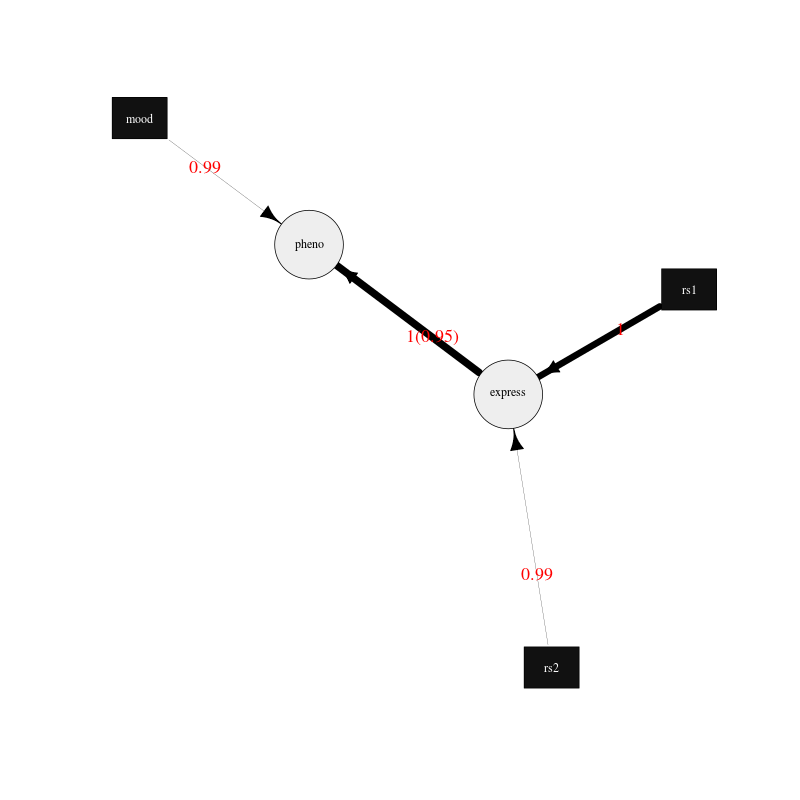
\includegraphics[width=400pt]{ave-graph-example.png}}
\caption{Plot of the average network drawn using the igraph R package.}
\label{plot-ave1-fig}
\end{center}}
\end{figure}
}

The edges are drawn proportional to the edge strength (but scaled to be between the minimum and maximum edge widths), that is, the proportion of best fit networks that the edge appears in after bootstrapping. Although using the \code{-average-networks-use-weight-method} option the strength can be weighted using the chi square values of each edge significance. The direction indicates the proportion of times the edge points in the given direction when it appears in a best fit network. The edges are labelled in red with the strength values followed by the direction values in brackets. Edges between discrete and continuous nodes do not have a direction value as they are constrained to be from the discrete node to the continuus node. The plot can easily be updated to your needs by following the igraphR package documentation. 

A graph may also be output to show the cumulative number of edges in the average network for different strength thresholds. If an edge has a strength greater than the strength threshold then it is included in the average network. 
{\begin{figure}[ht]
{\begin{center}
{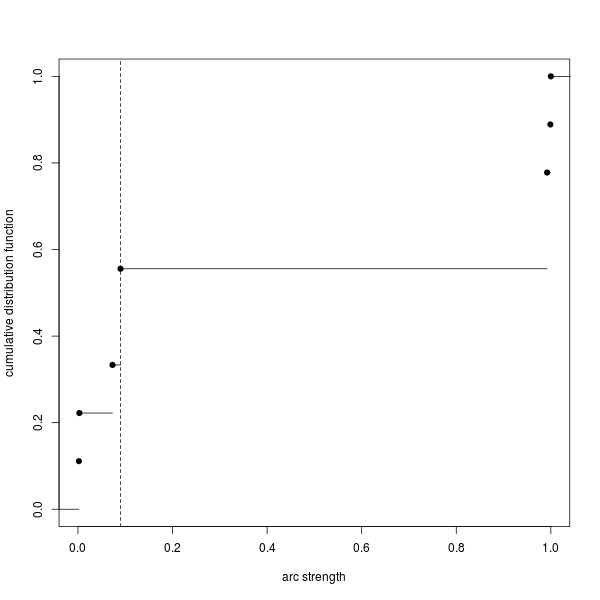
\includegraphics[width=400pt]{ave-graph-example-thresholdEst.png}}
\caption{Plot of the cumulative number of edges in the average network for different strength thresholds.}
\label{plot-ave2-fig}
\end{center}}
\end{figure}
}

%============ End of subsection "average-network-example"============

\subsection{Parallel Example}
\label{average-network-parallel}

As calculating the average network is a computationally intensive task, it makes sense it calculate it in parallel. This can be done by running the parallel version of BayesNetty as described in  section \ref{parallel}, but a much quicker way is given here by running the non-parallel version of BayesNetty in parallel and then combining the individual average network results in one final average network. 

The handy Unix script \code{runCalcAveNetPara} can be ran to do this as follows: 
\vspace{0.35cm} \begin{lstlisting}

./runCalcAveNetPara paras-average-parallel.txt average-network-example 20

\end{lstlisting} \vspace{0.35cm}
Where the first argument is a BayesNetty parameter file to calculate an average network, as below for example. The second argument is the file name of the average network to output, and the last argument is the number of processes to run in parallel. This will run 50 times 20 bootstraps (equal to 1000 bootstraps) overall to calculate the average network. 
\vspace{0.35cm} \begin{lstlisting}

#input continuous data
-input-data
-input-data-file example-cts.dat
-input-data-cts

#input discrete data
-input-data
-input-data-file example-discrete.dat
-input-data-discrete

#input SNP data as discrete data
-input-data
-input-data-file example.bed
-input-data-discrete-snp

#calculate average network
-average-networks
-average-networks-bootstraps 50

\end{lstlisting} \vspace{0.35cm}
The linux script \code{runCalcAveNetPara}, as shown below, runs a number of BayesNetty processes in parallel and sets different output files. As the random number seed is set by default by the execution time, and the processes are set off at the same time, it is necessary to set the seed to different values. The individual average networks are then combined using the \code{collate-average-nets.R} R script. Also, R code to plot the average graph is also output, which is modified for the appropriate threshold to plot the edges and the final average network file name. 
\vspace{0.35cm} \begin{lstlisting}

#!/bin/bash                                                                                                                                          

# $1 = parameter file to calculate average network in parallel                                                                                       
# $2 = average network file name                                                                                                                     
# $3 = no. of processes to run in parallel                                                                                                           

RANDOM=$$
#run bayesnetty $3 times for X bootstraps each                                                                                                       
#all processes are ran simultaneously in the background
for i in $(seq 1 $3);
do

./bayesnetty $1 -so -seed $i0$RANDOM -average-networks-file $2$i-i.dat -average-networks-igraph-file-prefix $2-graph&

done

#wait for all processes to finish                                                                                                                    
wait

#collate the results into a final average file                                                                                                       
R --vanilla --args $2 $3 < collate-average-nets.R

#delete individual average network files                                                                                                             
rm $2*-i.dat

#plot the final network                                                                                                                              
#set threshold                                                                                                                                       
t=$(cat "$2-threshold.dat")
sed -i "s/threshold<-/threshold<-$t #/g" $2-graph.R

#set final average file name                                                                                                                         
sed -i "s/aveGraph<-/aveGraph<-read.table(\"$2.dat\", header=TRUE, stringsAsFactors=FALSE) #/g" $2-graph.R

#plot average network                                                                                                                                
R --vanilla < $2-graph.R

\end{lstlisting} \vspace{0.35cm}
The R script \code{collate-average-nets.R} (used in the linux script above) combines the average networks and calculates a suggested threshold for plotting the network, as given below: 
\vspace{0.35cm} \begin{lstlisting}

#R file to collate average networks ran in parallel - all average networks must have been calculated with the same number of bootstraps
cmd_args<-commandArgs()

fileName<-cmd_args[4]
noFiles<-as.numeric(cmd_args[5])

totalNet<-read.table(paste(fileName,1,"-i.dat",sep=""), header=TRUE, stringsAsFactors=FALSE)

totalNet<-cbind(totalNet, rep(1, length(totalNet[,1])))
colnames(totalNet)[7]<-"count"

for(i in 2:noFiles)
{
   aveNet<-read.table(paste(fileName,i,"-i.dat",sep=""), header=TRUE, stringsAsFactors=FALSE)
   aveNet<-cbind(aveNet, rep(1, length(aveNet[,1])))
   colnames(aveNet)[7]<-"count"
   
   ##loop thro' rows of average table
   for(j in 1:length(aveNet[,1]))
   {
     ##find edge in total
     totRow<-which(aveNet$from[j]==totalNet$from & aveNet$to[j]==totalNet$to)
     if(length(totRow) == 1)
     {
         totalNet$strength[totRow]<-totalNet$strength[totRow] + aveNet$strength[j]
         totalNet$direction[totRow]<-totalNet$direction[totRow] + aveNet$direction[j]
         totalNet[totRow,7]<-totalNet[totRow,7]+1
     } else {
         totRow<-which(aveNet$from[j]==totalNet$to & aveNet$to[j]==totalNet$from)
         if(length(totRow) == 1)
         {
           totalNet$strength[totRow]<-totalNet$strength[totRow] + aveNet$strength[j]
           totalNet$direction[totRow]<-totalNet$direction[totRow] + 1 - aveNet$direction[j]
           totalNet[totRow,7]<-totalNet[totRow,7]+1
         } else {     
           totalNet<-rbind(totalNet, aveNet[j,])            
         }     
     }     
   }
}

##take average over all average networks
totalNet$strength<-totalNet$strength/noFiles
totalNet$direction<-totalNet$direction/totalNet[,7]

totalNet<-totalNet[order(-totalNet$strength),1:6]

#reorder edges if direction < 0.5
for(j in 1:length(totalNet[,1]))
{
   if(totalNet$direction[j] < 0.5)
   {
      totalNet[j,]<-c(totalNet$to[j], totalNet[j,2], totalNet$from[j], totalNet[j,4], totalNet[j,5], 1-as.numeric(totalNet[j,6]))
   }
}

write.table(totalNet, paste(fileName,".dat",sep=""), quote=FALSE, col.names=TRUE, row.names=FALSE)

#calculate suggested threshold for plotting network
cumCount = 0;
arcStrength = 0;
arcStrengths<-c()
cumArcStrengths<-c()
oas<-1
    
repeat
{
		arcStrength = rev(totalNet$strength)[oas];
		
		repeat
		{			
			oas<-oas+1
			cumCount<-cumCount+1

		 if(rev(totalNet$strength)[oas] > arcStrength || oas > length(rev(totalNet$strength))) break
    }
    
    if(length(arcStrengths) > 0 && arcStrength == arcStrengths[length(arcStrengths)])
    {
      arcStrengths[length(arcStrengths)]<-arcStrength
      cumArcStrengths[length(arcStrengths)]<-cumCount
    } else {
      arcStrengths<-append(arcStrengths, arcStrength)
      cumArcStrengths<-append(cumArcStrengths, cumCount)
    } 
     
     if(oas > length(rev(totalNet$strength))) break
}
 
bestL1score<-cumCount
propArcs<-cumArcStrengths/cumArcStrengths[length(cumArcStrengths)]

for(i in 1:length(arcStrengths)) #casTh in acumTot) 
{
    j<-1
		L1score = propArcs[i] *arcStrengths[1];
  
		prevCum = propArcs[j];
		prevStrength = arcStrengths[j];
		j<-j+1;

		while(j <= length(arcStrengths)) 
		{
			if(prevCum > propArcs[i]) L1score<-L1score + (prevCum - propArcs[i]) *(arcStrengths[j] - prevStrength)
			else L1score<-L1score + (propArcs[i] - prevCum) *(arcStrengths[j] - prevStrength)
			
			prevCum = propArcs[j];
			prevStrength = arcStrengths[j];
			j<-j+1
		}

		if(L1score < bestL1score)
		{
			bestL1score = L1score;
			bestThreshold = arcStrengths[i]
		}
}
 
write.table(bestThreshold, paste(fileName,"-threshold.dat",sep=""), quote=FALSE, col.names=FALSE, row.names=FALSE)

\end{lstlisting} \vspace{0.35cm}
The files \code{paras-average-parallel.txt}, \code{runCalcAveNetPara} and \code{collate-average-nets.R} can be found in the example.zipfile. 

%============ End of subsection "average-network-parallel"============


%================== End of section "average-network"==================

\section{Impute Data}
\label{impute-data}

When there is missing data, the standard approach is to remove every individual with missing data before performing any Bayesian network analysis, and this is the default behaviour. 

This can be wasteful and undesirable when there are many individuals with missing data, perhaps with only one variable missing, making imputation a natural choice. 

BayesNetty includes a new imputation method designed to increase the power to detect causal relationships whilst accounting for model uncertainty. This method uses a version of nearest neighbour imputation, whereby missing data from one individual is replaced with data from another individual, the nearest neighbour. 

An important feature of this approach is that it can be used with both discrete and continuous data. 

For each individual with missing data, subsets of variables that can be used to find the nearest neighbour are chosen by bootstrapping the complete data to estimate a Bayesian network. 
\subsection{Options}
\label{impute-data-options}

The options are as follows: 

{\begin{center}\resizebox{16cm}{!}{\begin{tabular}{lp{9cm}l}
Option  & Description  & Default\\
\hline
-impute-network-data  & do a task to impute network data  & \\
-impute-network-data-name name  & label the task with a name  & Task-n\\
-impute-network-data-network-name network  & the name of the network to impute data for  & previous network (or the default model given by a node for each data variable and no edges if there is no previous network)\\
-impute-network-data-min-non-missing-edges x  & the percentage (0 to 100) of non-missing edges required to impute data for an individual  & 0\\
-impute-network-data-random-restarts n  & for each bootstrap network fit do another n searches starting from a random network  & 0\\
-impute-network-data-jitter-restarts m  & for each bootstrap network fit after the initial search and every random restart search do another m searches jittered from the recently found network  & 0\\
-impute-network-data-start-indiv a  & start imputing data from individual a  & 1\\
-impute-network-data-end-indiv b  & end imputing data at individual b  & last individual\\
-impute-network-data-job i t  & only impute individuals for subset i from a total of t subsets  & \\
\end{tabular}}\end{center}}

The only option that is necessary to impute data is the \code{-impute-network-data} option. 

Once data has been imputed its missing data is filled in with imputed values and any subsequent analyses in BayesNetty will use this imputed data. 

If an individual has too much missing data then it may not be beneficial to impute the data for this individual, as the imputed data would be too poor to add value to any analysis. The \code{-impute-network-min-non-missing-edges} allows the user to change the required amount of edges between non-missing variables to impute data for an individual. Around {\bf 50} percent has been shown to be a suitable value to impute most individuals whilst effectively discarding individuals with too much missing data, although it may depend on the structure of any fitted networks. If this value is set to 0 then all individuals will have their data imputed, and a value of 100 will result in no data being imputed. If data set has a block of data with non-missing data for only a few variables then it is best to simply remove these individuals before using BayesNetty. 

The \code{-impute-network-data-random-restarts} and \code{-impute-network-data-jitter-restarts} options can be increased to improve the network search at each step of the algorithm and may potentially increase the quality of the imputed data at the expense of a longer running time. 

The \code{-impute-network-data-start-indiv}, \code{-impute-network-data-end-indiv} and \code{-impute-network-data-job} options may be used to only impute a range of individuals. These options may be useful for large networks to impute data in parallel and then combine later if the data is output to file (see  section \ref{output-network} to output data). See  section \ref{impute-parallel-example} for an example. 

The option \code{-impute-network-data-job} can also be used to only impute data for some individuals and makes it easier to split the imputation into a number of jobs. 

%============ End of subsection "impute-data-options"============

\subsection{Example}
\label{impute-example}

The following is an example parameter file to impute network data and search for the best network both before and after imputation. 
\vspace{0.35cm} \begin{lstlisting}

#input continuous data
-input-data
-input-data-file impute-example-cts.dat
-input-data-cts

#input SNP data as discrete data
-input-data
-input-data-file impute-example.bed
-input-data-discrete-snp

#search network models with the original data
-search-models

#impute the missing data
-impute-network-data

#search network models with the imputed data
-search-models

\end{lstlisting} \vspace{0.35cm}
This parameter file, \code{paras-impute.txt}, and example data for imputation can be found in impute-example.zipand can be used as follows: 
\vspace{0.35cm} \begin{lstlisting}

./bayesnetty paras-impute.txt

\end{lstlisting} \vspace{0.35cm}
Which should produce output that looks like something as follows: 
\vspace{0.35cm} \begin{lstlisting}

BayesNetty: Bayesian Network software, v1.00
--------------------------------------------------
Copyright 2015-present Richard Howey, GNU General Public License, v3
Institute of Genetic Medicine, Newcastle University

Random seed: 1545221384
--------------------------------------------------
Task name: Task-1
Loading data
Continuous data file: impute-example-cts.dat
Number of ID columns: 2
Including (all) 5 variables in analysis
Each variable has 1000 data entries
Missing value: not set
--------------------------------------------------
--------------------------------------------------
Task name: Task-2
Loading data
SNP binary data file: impute-example.bed
SNP data treated as discrete data
Total number of SNPs: 2
Total number of subjects: 1000
Number of ID columns: 2
Including (all) 2 variables in analysis
Each variable has 1000 data entries
--------------------------------------------------
--------------------------------------------------
Task name: Task-3
Searching network models
--------------------------------------------------
Loading defaultNetwork network
Network type: bnlearn
Network score type: BIC
Total number of nodes: 7 (Discrete: 2 | Factor: 0 | Continuous: 5)
Total number of edges: 0
Network Structure: [bio1][bio2][bio3][trait1][trait2][rs1][rs2]
Total data at each node: 213
Missing data at each node: 787
--------------------------------------------------
Network: defaultNetwork
Search: Greedy
Random restarts: 0
Random jitter restarts: 0
Network Structure: [rs1][rs2][trait2|rs2][bio2|trait2][trait1|bio2][bio1|trait1][bio3|bio1:bio2]
Network score type: BIC
Network score = -1970.2
--------------------------------------------------
--------------------------------------------------
Task name: Task-4
Imputing network data
Network: defaultNetwork
Network Structure: [rs1][rs2][trait2|rs2][bio2|trait2][trait1|bio2][bio1|trait1][bio3|bio1:bio2]
Number of individuals with missing data: 787
Number of individuals imputed: 787
Percentage of data imputed (when attempted): 98.4466
Minimum percentage of non-missing edges (or singleton nodes) required to impute individual: 50
Random restarts: 0
Random jitter restarts: 0
--------------------------------------------------
--------------------------------------------------
Task name: Task-5
Searching network models
Network: defaultNetwork
Search: Greedy
Random restarts: 0
Random jitter restarts: 0
Network Structure: [bio1][bio2][bio3|bio1:bio2][rs1][rs2][trait1|bio1:rs1][trait2|bio2:rs2]
Network score type: BIC
Network score = -9240.19
--------------------------------------------------

Run time: 34 seconds

\end{lstlisting} \vspace{0.35cm}
The data is loaded, a search is performed and then the network data is imputed and another search is performed. The run time for performing imputation is longer than most other operations in BayesNetty. This is because, every individual with missing data, we take a 90% sample (without replacement) of the individuals with complete data at the variables of interest. This sampled data set is used to find a best fit network. This best fit network determines the variables that are used to choose the nearest neighbour for the individual with missing data, and then the missing data is filled in from the nearest neighbour. 

There are a lot of individuals with missing data in this example data resulting in the incorrect network being estimated initially but after the data is imputed the correct network is found. That is, the network that the data was simulated from. 

It may be possible that some individuals are not imputed as they have too much missing data, or sometimes only partially imputed if the data is not suitable for the imputation algorithm. 

%============ End of subsection "impute-example"============

\subsection{Parallel Example}
\label{impute-parallel-example}

As imputing network data is a computationally intensive task, it makes sense to do it in parallel. This can be done by running the parallel version of BayesNetty as described in  section \ref{parallel}, but a much quicker way is given here by running the non-parallel version of BayesNetty in parallel where each process imputes a subset of the individuals. The data of the imputed individuals can then be output for each process (see  section \ref{output-network}) and then combined into the final imputed data set. 

A handy Unix script has been written to do this and is ran as follows: 
\vspace{0.35cm} \begin{lstlisting}

./runImputeParallel paras-impute-parallel.txt imputed-data 20

\end{lstlisting} \vspace{0.35cm}
The first argument is a Bayesnetty parameter file to impute the data (example shown below). The second argument is a file name (without extension) for the imputed data set to be outputted to. The last argument is the number of processes to run. 
\vspace{0.35cm} \begin{lstlisting}

#input continuous data
-input-data
-input-data-file impute-example-cts.dat
-input-data-cts

#input SNP data as discrete data
-input-data
-input-data-file impute-example.bed
-input-data-discrete-snp

#impute the missing data
-impute-network-data

#output the network data, set file names on command line
-output-network

\end{lstlisting} \vspace{0.35cm}
The Unix script \code{runImputeParallel}, as shown below, runs a number of BayesNetty processes in parallel and outputs separate data files for different subsets of individuals. As the random number seed is set by default by the execution time, and the processes are set off at the same time, it is necessary to set the seed to different values. The output files are then combined and the data files from separate processes deleted. 
\vspace{0.35cm} \begin{lstlisting}

#!/bin/bash                                                                                                                                                                                       
# $1 = parameter file to impute data in parallel
# $2 = imputed data file name
# $3 = no. of processes to run in parallel                                                                                                                                                       
RANDOM=$$
#run bayesnetty $3 times for X bootstraps each; processes run simultaneously in the background                                                                
for i in $(seq 1 $3);
do

./bayesnetty $1 -so -seed $i0$RANDOM -output-network-node-data-file-prefix $2$i-i -output-network-node-data-bed-file -output-network-node-data-job $i $3 -impute-network-data-job $i $3&

done

#wait for all processes to finish
wait

##collate files                                                                                                                                                                                   
if [ -f "$21-i-cts.dat" ]
then
 > $2-cts.dat
fi

if [ -f "$21-i-discrete.dat" ]
then
 > $2-discrete.dat
fi

for j in $(seq 1 $3);
do

#collate cts data
if [ -f "$2$j-i-cts.dat" ]
then
 cat $2$j-i-cts.dat >> $2-cts.dat
 rm $2$j-i-cts.dat
fi

#collate discrete data
if [ -f "$2$j-i-discrete.dat" ]
then
 cat $2$j-i-discrete.dat >> $2-discrete.dat
 rm $2$j-i-discrete.dat
fi


#collate SNP plink style data
if [ -f "$2$j-i.fam" ]
then

 if [ $j == 1 ]
 then
  cp $2$j-i.fam $2.fam
  cp $2$j-i.bim $2.bim
  cp $2$j-i.bed $2.bed
 else
  plink --noweb --silent --bfile $2 --bmerge $2$j-i.bed $2$j-i.bim $2$j-i.fam --make-bed --out $2-merge
  mv $2-merge.bed $2.bed
  mv $2-merge.bim $2.bim
  mv $2-merge.fam $2.fam
  rm $2-merge.log
 fi

 rm $2$j-i.fam
 rm $2$j-i.bim
 rm $2$j-i.bed
fi

done

\end{lstlisting} \vspace{0.35cm}
The final imputed data can then be used in any BayesNetty analysis. For example, to search for the best fit network: 
\vspace{0.35cm} \begin{lstlisting}

./bayesnetty paras-search-imputed-data.txt

\end{lstlisting} \vspace{0.35cm}
Where the parameter file is as follows: 
\vspace{0.35cm} \begin{lstlisting}

#input imputed continuous data
-input-data
-input-data-file imputed-data-cts.dat
-input-data-cts

#input imputed SNP data as discrete data
-input-data
-input-data-file imputed-data.bed
-input-data-discrete-snp

#search network models with the imputed data
-search-models

\end{lstlisting} \vspace{0.35cm}
The files \code{paras-impute-parallel.txt}, \code{runImputeParallel} and \code{paras-search-imputed-data.txt} can be found in the impute-example.zipfile. 

%============ End of subsection "impute-parallel-example"============


%================== End of section "impute-data"==================

\section{Estimate Imputation Benefit}
\label{estimate-impute}

For a given data set with missing data it is natural to wonder how much benefit imputation brings. We include an option in BayesNetty to attempt to compare different methods of fitting a best fit network to this data set. We use estimates of the recall and precision to compare the methods. The recall is the percentage of edges that were recovered from the simulation model and the precision is the percentage of edges in the fitted model that are in the simulation model. For an edge to be correct it must be in the correct direction. However, if the simulating network has equivalent networks such that some edges may be in either direction, then these edges are considered correct if they are in any direction. 

The method follows these steps: 
\begin{enumerate}

\item An initial network is fitted using imputation. 
\item Data is simulated using this network for the same number of individuals in the original data set. 
\item A best fit network is found for the full data set. 
\item The simulated data set has values set to missing as in the original data set. 
\item Best fit networks are found for this data set using: (i) a reduced data set with only complete data; (ii) data imputation; (iii) data imputation with complete training data. 
\item Recall and precision are calculated for the 4 different best fit networks against the simulation network.\end{enumerate}

This method can be repeated a number times as is computationally feasible to take average recall and precision estimates to account for variability in the simulated data. The recall and precision using the full data set gives an estimate of an upper limit of what may feasibly be achieved using data imputation. Comparing the recall and precision of the reduced data set with imputation gives an estimate of the increased benefit of using imputation. Comparing the two imputation methods should show when it is appropriate to use the variant imputation method. 

A major drawback of this estimation method is the obvious fact that we do not know the ``true'' network structure of the data, we therefore use an estimated network to simulate the data and hope this is sufficiently close for the results to be useful. In general, we have found that the benefits of imputation are often understated as the simulation network tends to be set without some of the weaker edges that cannot always be detected (when using data sets where we do actually know the ``true'' network). Even if we cannot be too sure of the exact gain in benefit of imputation this BayesNetty estimation method can give clear confidence of a benefit when there are large differences (and if the variant method using complete training data performs any better). 
\subsection{Options}
\label{estimate-impute-options}

The options are as follows: 

{\begin{center}\resizebox{16cm}{!}{\begin{tabular}{lp{9cm}l}
Option  & Description  & Default\\
\hline
-impute-estimate-recall-precision  & do a task to estimate recall and precision before and after data imputation\\
-impute-estimate-recall-precision name  & label the task with a name  & Task-n\\
-impute-estimate-recall-precision-network-name network  & set the name of the initial network when estimating recall and precision  & previous network (or the default model given by a node for each data variable and no edges if there is no previous network)\\
-impute-estimate-recall-precision-random-restarts n  & for each network fit do another n searches starting from a random network  & \\
-impute-estimate-recall-precision-jitter-restarts m  & for each network fit after the initial search and every random restart search do another m searches jittered from the recently found network  & 0\\
-impute-estimate-recall-precision-skip-imputation  & do not estimate recall and precision for imputed data  & \\
-impute-estimate-recall-precision-iterations i  & estimate the recall and precision i times and take the average  & 1\\
\end{tabular}}\end{center}}

%============ End of subsection "estimate-impute-options"============

\subsection{Example}
\label{estimate-impute-example}

An example of estimating the recall and precision is contained in the parameter file \code{paras-example-estimate-recall-precision.txt}, which can be found in example.zip.For simplicity the example is chosen to be a discrete network and this approach can be used for any kind of data. The network is the \code{child} network from the bnlearn repository \citet{bnlearn}. 
\vspace{0.35cm} \begin{lstlisting}

#input example data to estimate recall and precision from
-input-data
-input-data-file data-example-est-recall-precision.dat
-input-data-ids 0
-input-data-discrete

#set up network with no edges
-input-network
-input-network-empty

#estimate recall and precision for this data set
-impute-estimate-recall-precision
-impute-estimate-recall-precision-iterations 10
-impute-estimate-recall-precision-random-restarts 2
-impute-estimate-recall-precision-jitter-restarts 2

\end{lstlisting} \vspace{0.35cm}
This can be executed as usual 
\vspace{0.35cm} \begin{lstlisting}

./bayesnetty paras-example-estimate-recall-precision.txt

\end{lstlisting} \vspace{0.35cm}
and will output something as follows 
\vspace{0.35cm} \begin{lstlisting}

BayesNetty: Bayesian Network software, v1.1
--------------------------------------------------
Copyright 2015-present Richard Howey, GNU General Public License, v3
Institute of Genetic Medicine, Newcastle University

Random seed: 1605624192
--------------------------------------------------
Task name: Task-1
Loading data
Discrete data file: data-example-est-recall-precision.dat
Number of ID columns: 0
Including (all) 20 variables in analysis
Each variable has 500 data entries
Missing value: NA
--------------------------------------------------
--------------------------------------------------
Task name: Task-2
Loading network
Network set with no edges
Network type: bnlearn
Network score type: BIC
Total number of nodes: 20 (Discrete: 20 | Factor: 0 | Continuous: 0)
Total number of edges: 0
Network Structure: [Age][BirthAsphyxia][CO2Report][CO2][CardiacMixing][ChestXray][Disease][DuctFlow]
[GruntingReport][Grunting][HypDistrib][HypoxiaInO2][LVH][LVHreport][LowerBodyO2][LungFlow][LungParench][RUQO2][Sick][XrayReport]
Total data at each node: 54
Missing data at each node: 446
--------------------------------------------------
--------------------------------------------------
Task name: Task-3
Estimating the recall and precision when imputing network data
Network: Task-2
Number of iterations: 10
Random restarts: 2
Random jitter restarts: 2
Minimum percentage of non-missing edges (or singleton nodes) required to impute individual: 0
Individuals with data: 54
Individuals with missing data: 446

Recall: the percentage of edges found from the original true network
Precision: the percentage of edges in the network that are also in the original true network

                                   Recall     Precision
No imputation                      40.91      61.66
Imputation                         78.95      89.03
Imputation (complete training)     67.75      80.04
Full data (upper limit)            90.21      95.02

--------------------------------------------------

Run time: 1 hour, 39 minutes and 23 seconds

\end{lstlisting} \vspace{0.35cm}
From the example output we can see that with no imputation the recall is estimated to be 40.91 percent and the precision estimated to be is 61.66 percent, but if the full data were available it would be 90.21 and 95.02 respectively. Using our imputation method the estimated recall and precision is 78.95 and 89.03 respectively, which is quite a large increase. Our variant imputation method with complete training data also increases the recall and precision by quite a lot. 

Note that the estimation is stochastic due to the stochastic nature of the imputation method, and to a lesser extent the stochastic nature of finding a best fit model, and so rerunning the analyses may results in slightly different estimates. 

%============ End of subsection "estimate-impute-example"============


%================== End of section "estimate-impute"==================

\section{Calculate Recall and Precision}
\label{calc-recall-precision}

It is possible to calculate the recall and precision of a network against the ``true'' network structure. Typically this option will be used when the true network structure is chosen and used to simulate data. A best fit network can then be found for this data and the accuaracy assessed by calculating the recall and precision. 

For a network the recall is the percentage of edges found from the original true network. The precision is the percentage of edges in the network that are also in the original true network. For an edge to be correct it must be in the correct direction. However, if the true network has equivalent networks such that some edges may be in either direction, then these edges are considered correct if they are in either direction. 
\subsection{Options}
\label{calc-recall-precision-options}

The options are as follows: 

{\begin{center}\resizebox{16cm}{!}{\begin{tabular}{lp{9cm}l}
Option  & Description  & Default\\
\hline
-calculate-recall-precision  &  & \\
-calculate-recall-precision-name  & label the task with a name  & Task-n\\
-calculate-recall-precision-network-name network1  & the name of the network to calculate the recall and precision for  & \\
-calculate-recall-precision-true-network-name network2  & the name of the true network to calculate the recall and precision against  & \\
-calculate-recall-precision-file file.dat  & file to write recall and precision results to  & \\
\end{tabular}}\end{center}}

%============ End of subsection "calc-recall-precision-options"============

\subsection{Example}
\label{calc-recall-precision-example}

An example of calculating the recall and precision is contained in the parameter file \code{paras-example-calc-recall-precision.txt}, which can be found in example.zip.The network is again taken from the \code{child} network from the bnlearn repository \citet{bnlearn}. 

For example, the following parameter file: 
\vspace{0.35cm} \begin{lstlisting}

#input the network to calculate the recall and precision of
-input-network
-input-network-name example-net
-input-network-file example-net-calc-recall-pre.dat

#input true network structure for these nodes
-input-network
-input-network-name true-net
-input-network-file example-true-net-child.dat

#calculate the recall and precision
-calculate-recall-precision
-calculate-recall-precision-network-name example-net
-calculate-recall-precision-true-network-name true-net
-calculate-recall-precision-file recall-precision.dat

\end{lstlisting} \vspace{0.35cm}
can be ran in the usual way 
\vspace{0.35cm} \begin{lstlisting}

./bayesnetty paras-example-calc-recall-precision.txt

\end{lstlisting} \vspace{0.35cm}
and will output something as follows 
\vspace{0.35cm} \begin{lstlisting}

BayesNetty: Bayesian Network software, v1.1
--------------------------------------------------
Copyright 2015-present Richard Howey, GNU General Public License, v3
Institute of Genetic Medicine, Newcastle University

Random seed: 1605806239
--------------------------------------------------
Task name: example-net
Loading network
Network file: example-net-calc-recall-pre.dat
Network type: bnlearn
Network score type: BIC
Total number of nodes: 20 (Discrete: 0 | Factor: 0 | Continuous: 0 | No data: 20)
Total number of edges: 16
Network Structure: [BirthAsphyxia][LVHreport][RUQO2][Sick][XrayReport][Age|Sick]
[ChestXray|XrayReport][LVH|LVHreport][LowerBodyO2|LVHreport][CO2Report|Age]
[HypDistrib|LowerBodyO2][LungFlow|ChestXray][CO2|CO2Report][DuctFlow|LungFlow]
[Disease|DuctFlow][CardiacMixing|Disease][HypoxiaInO2|CardiacMixing][GruntingReport|Hy...
The network has nodes with no data
--------------------------------------------------
--------------------------------------------------
Task name: true-net
Loading network
Network file: example-true-net-child.dat
Network type: bnlearn
Network score type: BIC
Total number of nodes: 20 (Discrete: 0 | Factor: 0 | Continuous: 0 | No data: 20)
Total number of edges: 25
Network Structure: [BirthAsphyxia][Disease|BirthAsphyxia][CardiacMixing|Disease][DuctFlow|Disease]
[LVH|Disease][LungFlow|Disease][LungParench|Disease][Sick|Disease][Age|Disease:Sick][CO2|LungParench]
[ChestXray|LungFlow:LungParench][Grunting|LungParench:Sick][HypDistrib|CardiacMixing:DuctFlow][HypoxiaInO2|CardiacMixing...
The network has nodes with no data
--------------------------------------------------
--------------------------------------------------
Task name: Task-3
Calculating the recall and precision
Network: example-net
Network Structure: [BirthAsphyxia][LVHreport][RUQO2][Sick][XrayReport][Age|Sick][ChestXray|XrayReport]
[LVH|LVHreport][LowerBodyO2|LVHreport][CO2Report|Age][HypDistrib|LowerBodyO2][LungFlow|ChestXray]
[CO2|CO2Report][DuctFlow|LungFlow][Disease|DuctFlow][CardiacMixing|Disease][HypoxiaInO2|CardiacMixing][GruntingReport|Hy...
True Network: true-net
True Network Structure: [BirthAsphyxia][Disease|BirthAsphyxia][CardiacMixing|Disease][DuctFlow|Disease]
[LVH|Disease][LungFlow|Disease][LungParench|Disease][Sick|Disease][Age|Disease:Sick][CO2|LungParench]
[ChestXray|LungFlow:LungParench][Grunting|LungParench:Sick][HypDistrib|CardiacMixing:DuctFlow][HypoxiaInO2|CardiacMixing...
Recall and precision written to file: recall-precision.dat

Recall: the percentage of edges found from the original true network
Precision: the percentage of edges in the network that are also in the original true network

Recall: 32
Precision: 50

Recall and precision written to file: recall-precision.dat
--------------------------------------------------

Run time: less than one second

\end{lstlisting} \vspace{0.35cm}
In this example the network for which we wish we calculate the recall and precision is input into BayesNetty. The true network structure is then also input into BayesNetty. Finally the recall and precision is calculated and the results output to a file. This file simply contains 2 numbers: the recall followed by the precision. 

%============ End of subsection "calc-recall-precision-example"============


%================== End of section "calc-recall-precision"==================

\section{Simulate network data}
\label{sim-data}

It is possible to simulate data for a given network using BayesNetty. The network must be a bnlearn network, see  section \ref{bnlearn}, and can be set using a network file which has the same format as a posterior file and sets the network structure and the network parameters. Alternatively, rather than reading in a posterior file, the simulating network can be set by first (in the same parameter file) carrying out any analysis task in BayesNetty that results in a bnlearn network with calculated posteriors. 
\subsection{Options}
\label{sim-data-options}

The options are as follows: 

{\begin{center}\resizebox{16cm}{!}{\begin{tabular}{lp{9cm}l}
Option  & Description  & Default\\
\hline
-simulate-network-data  & do a task to simulate network data for a given network  & \\
-simulate-network-data-name name  & label the task with a name  & Task-n\\
-simulate-network-data-network-name network  & simulate data for this network  & previous network (or the default model given by a node for each data variable and no edges if there is no previous network)\\
-simulate-network-data-no-sims n  & simulate n replicates of network data  & 100\\
-simulate-network-data-parameter-file parameters.txt  & network with parameters in bnlearn posteriors file format  & \\
-simulate-network-data-whitelist-file whitelist.dat  & a list of edges that must be included in any network  & \\
-simulate-network-data-blacklist-file blacklist.dat  & a list of edges that must {\it not} be included in any network  & \\
-simulate-network-data-score score  & for a bnlearn network choose between loglike, AIC or BIC  & BIC\\
\end{tabular}}\end{center}}

%============ End of subsection "sim-data-options"============


If posteriors are not given then default network node parameters are used to simulate data. The default probabilities for a discrete SNP node are 0.25, 0.5 and 0.25 for levels 0, 1 and 2 respectively. A minor allele frequency of 0.5 would give these probabilites. For a discrete node the levels are given by equal probabilities. For a continuous node the intercept is set to 10 and the coefficients and variance are set to 1. 

The following sections show some examples of simulating data and can all be found in example.zip
\subsection{Example 1: no data}
\label{sim-data-example1}

This example simulates node data using a given network structure with network parameters. 

The network structure with network parameters must be given to simulate network data. These can be set by using a network parameters file which takes the same format as a posterior file and may be quite complex. To create this network parameter file it is therefore recommended to first output a posterior file for the network that you wish to simulate data for and then to edit this posterior file as required. 

To create a network parameter file, \code{example-network-parameters.txt}, run the parameter file, \code{paras-make-network-paras.txt}: 
\vspace{0.35cm} \begin{lstlisting}

#input the example network in format 1
-input-network
-input-network-file example-network-sim.dat

#simulate data using default parameters
-simulate-network-data

#calculate the posterior of the network using default parameters
-calc-posterior

#output the posteriors to be used as a network parameters file
-output-posteriors
-output-posteriors-file example-network-parameters.txt

\end{lstlisting} \vspace{0.35cm}
The example network file, \code{example-network-sim.dat}, is in network format 1, see  section \ref{input-network-formats}, except that extra (optional) node information is given as there is no node data to determine the node type. After each node either \code{|dis.snp}, \code{|cts.snp}, \code{|dis|2} or \code{|cts} may be written to give a discrete SNP node, a continuous SNP node, a discrete node with the number of levels or a continuous node respectively. If the type of node is not set then the node is set to a continuous node. If a discrete node is specified without the number of levels then the number of levels is set to 0. The example network file is as follows. 
\vspace{0.35cm} \begin{lstlisting}

rs1|dis.snp
rs2|dis.snp
mood|dis|2
express|cts
pheno|cts
rs1 pheno
rs2 pheno
mood express
pheno express

\end{lstlisting} \vspace{0.35cm}
The network parameter file, \code{example-network-parameters.txt}, can then be created by running the parameter file 
\vspace{0.35cm} \begin{lstlisting}

./bayesnetty paras-make-network-paras.txt

\end{lstlisting} \vspace{0.35cm}
The output will look something as follows 
\vspace{0.35cm} \begin{lstlisting}

BayesNetty: Bayesian Network software, v1.00
--------------------------------------------------
Copyright 2015-present Richard Howey, GNU General Public License, v3
Institute of Genetic Medicine, Newcastle University

Random seed: 1551712417
--------------------------------------------------
Task name: Task-1
Loading network
Network file: example-network-sim.dat
Network type: bnlearn
Network score type: BIC
Total number of nodes: 5 (Discrete: 0 | Factor: 0 | Continuous: 0 | No data: 5)
Total number of edges: 4
Network Structure: [rs1][rs2][mood][pheno|rs1:rs2][express|mood:pheno]
The network has nodes with no data
--------------------------------------------------
--------------------------------------------------
Task name: Task-2
Simulating network data
Data simulation network given by network: Task-1
Number of simulations: 100
Network: Task-2
Network type: bnlearn
Network score type: BIC
Total number of nodes: 5 (Discrete: 3 | Factor: 0 | Continuous: 2)
Total number of edges: 4
Network Structure: [rs1][rs2][mood][pheno|rs1:rs2][express|mood:pheno]
Total data at each node: 100
Missing data at each node: 0
--------------------------------------------------
--------------------------------------------------
Task name: Task-3
Calculating network score
Network: Task-2
Network structure: [rs1][rs2][mood][pheno|rs1:rs2][express|mood:pheno]
Network score type: BIC
Network score = -600.611
--------------------------------------------------
--------------------------------------------------
Task name: Task-4
Outputting posteriors
Network: Task-2
Network Structure: [rs1][rs2][mood][pheno|rs1:rs2][express|mood:pheno]
Output posteriors to file: example-network-parameters.txt
--------------------------------------------------

Run time: less than one second

\end{lstlisting} \vspace{0.35cm}
The network parameter file, \code{example-network-parameters.txt}, will look something like as follows: 
\vspace{0.35cm} \begin{lstlisting}

Posteriors:
===========

DISCRETE SNP NODE: rs1
  0: 0.26
  1: 0.49
  2: 0.25

DISCRETE SNP NODE: rs2
  0: 0.25
  1: 0.51
  2: 0.24

DISCRETE NODE: mood
  0: 0.47
  1: 0.53

CONTINUOUS NODE: express
 DISCRETE PARENTS: mood
 0:
  Intercept: 9.71024
  Coefficients: pheno: 1.04254 
  Mean: 20.2202
  Variance: 0.811076
 1:
  Intercept: 9.89
  Coefficients: pheno: 1.00832 
  Mean: 19.9452
  Variance: 0.6773

CONTINUOUS NODE: pheno
 DISCRETE PARENTS: rs1:rs2
 0:0:
  Intercept: 10.4619
  Coefficients: 
  Mean: 10.4619
  Variance: 2.07491
 1:0:
  Intercept: 9.97966
  Coefficients: 
  Mean: 9.97966
  Variance: 1.7134
 2:0:
  Intercept: 9.58534
  Coefficients: 
  Mean: 9.58534
  Variance: 0.532354
 0:1:
  Intercept: 10.0514
  Coefficients: 
  Mean: 10.0514
  Variance: 1.44765
 1:1:
  Intercept: 9.96623
  Coefficients: 
  Mean: 9.96623
  Variance: 0.760351
 2:1:
  Intercept: 9.54098
  Coefficients: 
  Mean: 9.54098
  Variance: 0.559675
 0:2:
  Intercept: 10.7559
  Coefficients: 
  Mean: 10.7559
  Variance: 1.78883
 1:2:
  Intercept: 10.1066
  Coefficients: 
  Mean: 10.1066
  Variance: 0.983235
 2:2:
  Intercept: 10.3842
  Coefficients: 
  Mean: 10.3842
  Variance: 1.50665

\end{lstlisting} \vspace{0.35cm}
The data was simulated using default network node parameters. The simulated node data and subsequent fitted parameters are thus close to these values. 

The network parameter file, \code{example-network-parameters.txt}, can now be edited using parameters of your choice. The mean is not required, this simply reports the mean of the node data for continuous nodes. The ``Posteriors'' title in the file is also not required, but these may be left in the file. The levels of discrete nodes are labelled 0, 1, 2 etc. These may be renamed to something more meaningful in this file. For example, for node ``mood'' the levels could be renamed ``sad'' and ``happy''. 

Finally, network node data may be simulated for a network with chosen network parameters where initially there was no data available for the network. 
\vspace{0.35cm} \begin{lstlisting}

#simulate data
-simulate-network-data
-simulate-network-data-no-sims 200
-simulate-network-data-parameter-file example-network-parameters.txt

#output simulated data
-output-network
-output-network-node-data-file-prefix sim-data
-output-network-node-data-bed-file

\end{lstlisting} \vspace{0.35cm}
The parameter file shown above, \code{paras-sim-data1.txt}, can then be used to simulate data and output it to several data files. 
\vspace{0.35cm} \begin{lstlisting}

./bayesnetty paras-sim-data1.txt

\end{lstlisting} \vspace{0.35cm}
The output will look something as follows 
\vspace{0.35cm} \begin{lstlisting}

BayesNetty: Bayesian Network software, v1.00
--------------------------------------------------
Copyright 2015-present Richard Howey, GNU General Public License, v3
Institute of Genetic Medicine, Newcastle University

Random seed: 1551712579
--------------------------------------------------
Task name: Task-1
Simulating network data
Number of simulations: 200
Parameter file name: example-network-parameters.txt
Network: Task-1
Network type: bnlearn
Network score type: BIC
Total number of nodes: 5 (Discrete: 3 | Factor: 0 | Continuous: 2)
Total number of edges: 4
Network Structure: [rs1][rs2][mood][pheno|rs1:rs2][express|mood:pheno]
Total data at each node: 200
Missing data at each node: 0
--------------------------------------------------
--------------------------------------------------
Task name: Task-2
Outputting network
Network: Task-1
Network Structure: [rs1][rs2][mood][pheno|rs1:rs2][express|mood:pheno]
Network output to file: network.dat
Node data output to files:
 sim-data-discrete.dat
 sim-data-cts.dat
 sim-data.bed/.bim/.fam
--------------------------------------------------

Run time: less than one second

\end{lstlisting} \vspace{0.35cm}
The file \code{sim-data-discrete.dat} contains the discrete node data, \code{sim-data-cts.dat} the continuous node data and \code{sim-data.bed}, \code{sim-data.bim} and \code{sim-data.fam} the SNP node data in PLINK binary pedigree format. 

%============ End of subsection "sim-data-example1"============

\subsection{Example 2: data and fitted network}
\label{sim-data-example2}

This example inputs some data, sets the network structure, fits network posterior parameters and then simulates network node data using these parameters. The simulated data is then output to file. The parameter file, \code{paras-sim-data2.txt}, in the example files does this and is as follows: 
\vspace{0.35cm} \begin{lstlisting}

#input continuous data
-input-data
-input-data-file example-cts.dat
-input-data-cts

#input discrete data
-input-data
-input-data-file example-discrete.dat
-input-data-discrete

#input SNP data as discrete data
-input-data
-input-data-file example.bed
-input-data-discrete-snp

#input the example network in format 1
-input-network
-input-network-file example-network-format1.dat

#simulate data
-simulate-network-data
-simulate-network-data-no-sims 200

#output simulated data
-output-network
-output-network-node-data-file-prefix sim-data
-output-network-node-data-bed-file

\end{lstlisting} \vspace{0.35cm}\vspace{0.35cm} \begin{lstlisting}

./bayesnetty paras-sim-data2.txt

\end{lstlisting} \vspace{0.35cm}
The output will look something as follows 
\vspace{0.35cm} \begin{lstlisting}

BayesNetty: Bayesian Network software, v1.00
--------------------------------------------------
Copyright 2015-present Richard Howey, GNU General Public License, v3
Institute of Genetic Medicine, Newcastle University

Random seed: 1551716397
--------------------------------------------------
Task name: Task-1
Loading data
Continuous data file: example-cts.dat
Number of ID columns: 2
Including (all) 2 variables in analysis
Each variable has 1500 data entries
Missing value: not set
--------------------------------------------------
--------------------------------------------------
Task name: Task-2
Loading data
Discrete data file: example-discrete.dat
Number of ID columns: 2
Including the 1 and only variable in analysis
Each variable has 1500 data entries
Missing value: NA
--------------------------------------------------
--------------------------------------------------
Task name: Task-3
Loading data
SNP binary data file: example.bed
SNP data treated as discrete data
Total number of SNPs: 2
Total number of subjects: 1500
Number of ID columns: 2
Including (all) 2 variables in analysis
Each variable has 1500 data entries
--------------------------------------------------
--------------------------------------------------
Task name: Task-4
Loading network
Network file: example-network-format1.dat
Network type: bnlearn
Network score type: BIC
Total number of nodes: 5 (Discrete: 3 | Factor: 0 | Continuous: 2)
Total number of edges: 4
Network Structure: [mood][rs1][rs2][pheno|rs1:rs2][express|pheno:mood]
Total data at each node: 1495
Missing data at each node: 5
--------------------------------------------------
--------------------------------------------------
Task name: Task-5
Simulating network data
Data simulation network given by network: Task-4
Number of simulations: 200
Network: Task-5
Network type: bnlearn
Network score type: BIC
Total number of nodes: 5 (Discrete: 3 | Factor: 0 | Continuous: 2)
Total number of edges: 4
Network Structure: [mood][rs1][rs2][pheno|rs1:rs2][express|pheno:mood]
Total data at each node: 200
Missing data at each node: 0
--------------------------------------------------
--------------------------------------------------
Task name: Task-6
Outputting network
Network: Task-5
Network Structure: [mood][rs1][rs2][pheno|rs1:rs2][express|pheno:mood]
Network output to file: network.dat
Node data output to files:
 sim-data-discrete.dat
 sim-data-cts.dat
 sim-data.bed/.bim/.fam
--------------------------------------------------

Run time: less than one second

\end{lstlisting} \vspace{0.35cm}
As in the previous example the simulated node data is output to a number of files. 

%============ End of subsection "sim-data-example2"============

\subsection{Example 3: data and unknown network}
\label{sim-data-example3}

In this example the network that the data will be simulated for is not known initially. To do this, some data is input, the best fitting network is chosen using a network search and then node data is simulated using the fitted parameters. The parameter file, \code{paras-sim-data3.txt}, in the example files does this and is as follows: 
\vspace{0.35cm} \begin{lstlisting}

#input continuous data
-input-data
-input-data-file example-cts.dat
-input-data-cts

#input discrete data
-input-data
-input-data-file example-discrete.dat
-input-data-discrete

#input SNP data as discrete data
-input-data
-input-data-file example.bed
-input-data-discrete-snp

#search for the best fitting model
-search-models

#simulate data
-simulate-network-data
-simulate-network-data-no-sims 200

#output simulated data
-output-network
-output-network-node-data-file-prefix sim-data
-output-network-node-data-bed-file

\end{lstlisting} \vspace{0.35cm}\vspace{0.35cm} \begin{lstlisting}

./bayesnetty paras-sim-data3.txt

\end{lstlisting} \vspace{0.35cm}
The output will look something as follows 
\vspace{0.35cm} \begin{lstlisting}

BayesNetty: Bayesian Network software, v1.00
--------------------------------------------------
Copyright 2015-present Richard Howey, GNU General Public License, v3
Institute of Genetic Medicine, Newcastle University

Random seed: 1551716718
--------------------------------------------------
Task name: Task-1
Loading data
Continuous data file: example-cts.dat
Number of ID columns: 2
Including (all) 2 variables in analysis
Each variable has 1500 data entries
Missing value: not set
--------------------------------------------------
--------------------------------------------------
Task name: Task-2
Loading data
Discrete data file: example-discrete.dat
Number of ID columns: 2
Including the 1 and only variable in analysis
Each variable has 1500 data entries
Missing value: NA
--------------------------------------------------
--------------------------------------------------
Task name: Task-3
Loading data
SNP binary data file: example.bed
SNP data treated as discrete data
Total number of SNPs: 2
Total number of subjects: 1500
Number of ID columns: 2
Including (all) 2 variables in analysis
Each variable has 1500 data entries
--------------------------------------------------
--------------------------------------------------
Task name: Task-4
Searching network models
--------------------------------------------------
Loading defaultNetwork network
Network type: bnlearn
Network score type: BIC
Total number of nodes: 5 (Discrete: 3 | Factor: 0 | Continuous: 2)
Total number of edges: 0
Network Structure: [express][pheno][mood][rs1][rs2]
Total data at each node: 1495
Missing data at each node: 5
--------------------------------------------------
Network: defaultNetwork
Search: Greedy
Random restarts: 0
Random jitter restarts: 0
Network Structure: [mood][rs1][rs2][express|rs1:rs2][pheno|express:mood]
Network score type: BIC
Network score = -8213.45
--------------------------------------------------
--------------------------------------------------
Task name: Task-5
Simulating network data
Data simulation network given by network: defaultNetwork
Number of simulations: 200
Network: Task-5
Network type: bnlearn
Network score type: BIC
Total number of nodes: 5 (Discrete: 3 | Factor: 0 | Continuous: 2)
Total number of edges: 4
Network Structure: [mood][rs1][rs2][express|rs1:rs2][pheno|express:mood]
Total data at each node: 200
Missing data at each node: 0
--------------------------------------------------
--------------------------------------------------
Task name: Task-6
Outputting network
Network: Task-5
Network Structure: [mood][rs1][rs2][express|rs1:rs2][pheno|express:mood]
Network output to file: network.dat
Node data output to files:
 sim-data-discrete.dat
 sim-data-cts.dat
 sim-data.bed/.bim/.fam
--------------------------------------------------

Run time: less than one second

\end{lstlisting} \vspace{0.35cm}
As in the previous example the simulated node data is output to a number of files. 

%============ End of subsection "sim-data-example3"============


%================== End of section "sim-data"==================

\section{Markov blanket}
\label{markov-blanket}

The Markov blanket for a node contains all the variables that shield the node from the rest of the network. This means that the Markov blanket of a node is the only knowledge needed to predict the behaviour of that node and its children. This may be useful for large networks where some nodes are of particular interest. See \citet{bnlearn} for more details. 

The \code{-markov-blanket} option can be used to calculate the Markov blanket for a given node. A sub-network is created for the given node and its Markov blanket which may be output using the \code{-output-network} option, see  section \ref{output-network}, or used in any other network analysis. 
\subsection{Options}
\label{markov-blanket-options}

The options are as follows: 

{\begin{center}\resizebox{16cm}{!}{\begin{tabular}{lp{9cm}l}
Option  & Description  & Default\\
\hline
-markov-blanket  & do a task to calculate the Markov blanket for a given node  & \\
-markov-blanket-name name  & label the task with a name  & Task-n\\
-markov-blanket-network-name network  & the name of the network to calculate the Markov blanket  & previous network (or the default model given by a node for each data variable and no edges if there is no previous network)\\
-markov-blanket-node-name node  & calculate the Markov blanket for the node with this name  & \\
\end{tabular}}\end{center}}

%============ End of subsection "markov-blanket-options"============

\subsection{Example}
\label{calc-blanket-example}

The Markov blanket for a given node is calculated by using the \code{-markov-blanket} option together with the \code{-markov-blanket-node-name} option to choose the node. For example: 
\vspace{0.35cm} \begin{lstlisting}

#input the example network
-input-network
-input-network-file example-network-format1.dat

#calculate the Markov Blanket
-markov-blanket
-markov-blanket-node-name express

#output the network
-output-network
-output-network-file express-markov-blanket.dat

\end{lstlisting} \vspace{0.35cm}
As the Markov blanket does not depend on the data of the nodes it is possible to calculate the Markov blanket without data. In the example the network structure is input, the Markov blanket calculated for the ``express'' node and then output to the file \code{express-markov-blanket.dat}. This parameter file, \code{paras-blanket.txt}, can be found in example.zipand produces output which should look something as follows: 
\vspace{0.35cm} \begin{lstlisting}

BayesNetty: Bayesian Network software, v1.00
--------------------------------------------------
Copyright 2015-present Richard Howey, GNU General Public License, v3
Institute of Genetic Medicine, Newcastle University

Random seed: 1551956198
--------------------------------------------------
Task name: Task-1
Loading network
Network file: example-network-format1.dat
Network type: bnlearn
Network score type: BIC
Total number of nodes: 5 (Discrete: 0 | Factor: 0 | Continuous: 0 | No data: 5)
Total number of edges: 4
Network Structure: [rs1][rs2][mood][pheno|rs1:rs2][express|mood:pheno]
The network has nodes with no data
--------------------------------------------------
--------------------------------------------------
Task name: Task-2
Calculating Markov blanket
Network: Task-1
Node: express
Network structure: [rs1][rs2][mood][pheno|rs1:rs2][express|mood:pheno]
Markov blanket network structure: [mood][pheno][express|mood:pheno]
--------------------------------------------------
--------------------------------------------------
Task name: Task-3
Outputting network
Network: Task-2
Network Structure: [mood][pheno][express|mood:pheno]
Network output to file: express-markov-blanket.dat
--------------------------------------------------

Run time: less than one second

\end{lstlisting} \vspace{0.35cm}
%============ End of subsection "calc-blanket-example"============


%================== End of section "markov-blanket"==================

\section{Output network}
\label{output-network}

A network may be output using the \code{-output-network} task. The network may be output in one of three different formats. The \code{-output-network-igraph-file-prefix} option can also be used to output igraph files, see  section \ref{plot-network} for more details. 

The output network task can also be used to output node data using the \code{-output-network-node-data-file-prefix} option and optionally the \code{-output-network-node-data-bed-file} option. 
\subsection{Options}
\label{output-network-options}

The options are as follows: 

{\begin{center}\resizebox{16cm}{!}{\begin{tabular}{lp{9cm}l}
Option  & Description  & Default\\
\hline
-output-network  & do a task to output a network to file  & \\
-output-network-name name  & label the task with a name  & Task-n\\
-output-network-network-name network  & output this network  & previous network (or the default model given by a node for each data variable and no edges if there is no previous network)\\
-output-network-file network.dat  & output the network in a format where the nodes and then the edges are listed  & \\
-output-network-file2 network2.dat  & output the network in this style of format: \code{[a][b|a][c|a:b]}  & \\
-output-network-equivalent-networks-file equiv-networks.dat  & output a list of equivalent networks to file equiv-networks.dat  & \\
-output-network-igraph-file-prefix mygraph  & output igraph format files consisting of mygraph-nodes.dat, mygraph-edges.dat and R code mygraph-plot.R  & \\
-output-network-node-data-file-prefix mydata  & output network discrete data to mydata-discrete.dat and continuous data to mydata-cts.dat  & \\
-output-network-node-data-bed-file  & output SNP data to files mydata.bed, mydata.bim and mydata.fam and not to files mydata-discrete.dat and mydata-cts.dat  & \\
-output-network-node-data-start-indiv a  & start output of data from individual a  & 1\\
-output-network-node-data-end-indiv b  & stop output of data at individual b  & last individual\\
-output-network-node-data-job i t  & only output individuals for subset i from a total of t subsets  & \\
\end{tabular}}\end{center}}

%============ End of subsection "output-network-options"============

\subsection{Example}
\label{output-network-example}

The following is an example parameter file to output a network. 
\vspace{0.35cm} \begin{lstlisting}

#input continuous data
-input-data
-input-data-file example-cts.dat
-input-data-cts

#input discrete data
-input-data
-input-data-file example-discrete.dat
-input-data-discrete

#input SNP data as discrete data
-input-data
-input-data-file example.bed
-input-data-discrete-snp

#search network models
-search-models

#output the fitted network
-output-network
-output-network-file fittedNetwork.dat

\end{lstlisting} \vspace{0.35cm}
This parameter file, \code{paras-output-network.txt}, can be found in example.zipand can be used as follows: 
\vspace{0.35cm} \begin{lstlisting}

./bayesnetty paras-output-network.txt

\end{lstlisting} \vspace{0.35cm}
Which should produce output that looks like something as follows: 
\vspace{0.35cm} \begin{lstlisting}

BayesNetty: Bayesian Network software, v1.00
--------------------------------------------------
Copyright 2015-present Richard Howey, GNU General Public License, v3
Institute of Genetic Medicine, Newcastle University

Random seed: 1551716789
--------------------------------------------------
Task name: Task-1
Loading data
Continuous data file: example-cts.dat
Number of ID columns: 2
Including (all) 2 variables in analysis
Each variable has 1500 data entries
Missing value: not set
--------------------------------------------------
--------------------------------------------------
Task name: Task-2
Loading data
Discrete data file: example-discrete.dat
Number of ID columns: 2
Including the 1 and only variable in analysis
Each variable has 1500 data entries
Missing value: NA
--------------------------------------------------
--------------------------------------------------
Task name: Task-3
Loading data
SNP binary data file: example.bed
SNP data treated as discrete data
Total number of SNPs: 2
Total number of subjects: 1500
Number of ID columns: 2
Including (all) 2 variables in analysis
Each variable has 1500 data entries
--------------------------------------------------
--------------------------------------------------
Task name: Task-4
Searching network models
--------------------------------------------------
Loading defaultNetwork network
Network type: bnlearn
Network score type: BIC
Total number of nodes: 5 (Discrete: 3 | Factor: 0 | Continuous: 2)
Total number of edges: 0
Network Structure: [express][pheno][mood][rs1][rs2]
Total data at each node: 1495
Missing data at each node: 5
--------------------------------------------------
Network: defaultNetwork
Search: Greedy
Random restarts: 0
Random jitter restarts: 0
Network Structure: [mood][rs1][rs2][express|rs1:rs2][pheno|express:mood]
Network score type: BIC
Network score = -8213.45
--------------------------------------------------
--------------------------------------------------
Task name: Task-5
Outputting network
Network: defaultNetwork
Network Structure: [mood][rs1][rs2][express|rs1:rs2][pheno|express:mood]
Network output to file: fittedNetwork.dat
--------------------------------------------------

Run time: less than one second

\end{lstlisting} \vspace{0.35cm}
The data is loaded, a search is performed and then the network is output to a file. 

%============ End of subsection "output-network-example"============


%================== End of section "output-network"==================

\section{Output priors (deal only)}
\label{output-priors}

The priors for a deal network may be output to file for inspection with the \code{-output-priors}. The deal Bayesian network model has a quite complex default prior which is based on the given network data, structure and imaginary sample size, see \citet{deal} for details. The bnlearn Bayesian network, which is the recommended and default Bayesian network model, has no prior to output, see \citet{bnlearn} for details. 
\subsection{Options}
\label{output-priors-options}

The options are as follows: 

{\begin{center}\resizebox{16cm}{!}{\begin{tabular}{lp{9cm}l}
Option  & Description  & Default\\
\hline
-output-priors  & do a task to output the priors of a network to file  & \\
-output-priors-name name  & label the task with a name  & Task-n\\
-output-priors-network-name network  & output priors for this network  & previous network (or the default model given by a node for each data variable and no edges if there is no previous network)\\
-output-priors-file priors.dat  & output the priors to file priors.dat  & priors.dat\\
\end{tabular}}\end{center}}

%============ End of subsection "output-priors-options"============

\subsection{Example}
\label{output-priors-example}

The following is an example parameter file to output the priors of a network. 
\vspace{0.35cm} \begin{lstlisting}

#input continuous data
-input-data
-input-data-file example-cts.dat
-input-data-cts

#input discrete data
-input-data
-input-data-file example-discrete.dat
-input-data-discrete

#input SNP data as discrete data
-input-data
-input-data-file example.bed
-input-data-discrete-snp

#input the example network in format 1
-input-network
-input-network-file example-network-format1.dat
-input-network-type deal

#output the priors to file
-output-priors
-output-priors-file example-priors.dat

\end{lstlisting} \vspace{0.35cm}
This parameter file, \code{paras-output-priors.txt}, can be found in example.zipand can be used as follows: 
\vspace{0.35cm} \begin{lstlisting}

./bayesnetty paras-output-priors.txt

\end{lstlisting} \vspace{0.35cm}
Which should produce output that looks like something as follows: 
\vspace{0.35cm} \begin{lstlisting}

BayesNetty: Bayesian Network software, v1.00
--------------------------------------------------
Copyright 2015-present Richard Howey, GNU General Public License, v3
Institute of Genetic Medicine, Newcastle University

Random seed: 1551957572
--------------------------------------------------
Task name: Task-1
Loading data
Continuous data file: example-cts.dat
Number of ID columns: 2
Including (all) 2 variables in analysis
Each variable has 1500 data entries
Missing value: not set
--------------------------------------------------
--------------------------------------------------
Task name: Task-2
Loading data
Discrete data file: example-discrete.dat
Number of ID columns: 2
Including the 1 and only variable in analysis
Each variable has 1500 data entries
Missing value: NA
--------------------------------------------------
--------------------------------------------------
Task name: Task-3
Loading data
SNP binary data file: example.bed
SNP data treated as discrete data
Total number of SNPs: 2
Total number of subjects: 1500
Number of ID columns: 2
Including (all) 2 variables in analysis
Each variable has 1500 data entries
--------------------------------------------------
--------------------------------------------------
Task name: Task-4
Loading network
Network file: example-network-format1.dat
Network type: deal
Total number of nodes: 5 (Discrete: 3 | Factor: 0 | Continuous: 2)
Total number of edges: 4
Network Structure: [mood][rs1][rs2][pheno|rs1:rs2][express|pheno:mood]
Imaginary sample size: 10
Total data at each node: 1495
Missing data at each node: 5
--------------------------------------------------
--------------------------------------------------
Task name: Task-5
Outputting priors
Network: Task-4
Network Structure: [mood][rs1][rs2][pheno|rs1:rs2][express|pheno:mood]
Output priors to file: example-priors.dat
--------------------------------------------------

Run time: less than one second

\end{lstlisting} \vspace{0.35cm}
The data is loaded, the network input and then the prior is output to a file. 

%============ End of subsection "output-priors-example"============


%================== End of section "output-priors"==================

\section{Output posteriors}
\label{output-posteriors}

The posteriors may be output to file for inspection with the \code{-output-posteriors}. 
\subsection{Options}
\label{output-posteriors-options}

The options are as follows: 

{\begin{center}\resizebox{16cm}{!}{\begin{tabular}{lp{9cm}l}
Option  & Description  & Default\\
\hline
-output-posteriors  & do a task to output the posteriors of a network to file  & \\
-output-posteriors-name name  & label the task with a name  & Task-n\\
-output-posteriors-network-name network  & output posteriors for this network  & previous network (or the default model given by a node for each data variable and no edges if there is no previous network)\\
-output-posteriors-file posts.dat  & output the posteriors to file posts.dat  & posteriors.dat\\
\end{tabular}}\end{center}}

%============ End of subsection "output-posteriors-options"============

\subsection{Example}
\label{output-posts-example}

The following is an example parameter file to output the posteriors of a network. 
\vspace{0.35cm} \begin{lstlisting}

#input continuous data
-input-data
-input-data-file example-cts.dat
-input-data-cts

#input discrete data
-input-data
-input-data-file example-discrete.dat
-input-data-discrete

#input SNP data as discrete data
-input-data
-input-data-file example.bed
-input-data-discrete-snp

#input the example network in format 1
-input-network
-input-network-file example-network-format1.dat

#calculate the posterior of the network
-calc-posterior

#output the posteriors to file
-output-posteriors
-output-posteriors-file example-posteriors.dat

\end{lstlisting} \vspace{0.35cm}
This parameter file, \code{paras-output-post.txt}, can be found in example.zipand can be used as follows: 
\vspace{0.35cm} \begin{lstlisting}

./bayesnetty paras-output-post.txt

\end{lstlisting} \vspace{0.35cm}
Which should produce output that looks like something as follows: 
\vspace{0.35cm} \begin{lstlisting}

BayesNetty: Bayesian Network software, v1.00
--------------------------------------------------
Copyright 2015-present Richard Howey, GNU General Public License, v3
Institute of Genetic Medicine, Newcastle University

Random seed: 1551958097
--------------------------------------------------
Task name: Task-1
Loading data
Continuous data file: example-cts.dat
Number of ID columns: 2
Including (all) 2 variables in analysis
Each variable has 1500 data entries
Missing value: not set
--------------------------------------------------
--------------------------------------------------
Task name: Task-2
Loading data
Discrete data file: example-discrete.dat
Number of ID columns: 2
Including the 1 and only variable in analysis
Each variable has 1500 data entries
Missing value: NA
--------------------------------------------------
--------------------------------------------------
Task name: Task-3
Loading data
SNP binary data file: example.bed
SNP data treated as discrete data
Total number of SNPs: 2
Total number of subjects: 1500
Number of ID columns: 2
Including (all) 2 variables in analysis
Each variable has 1500 data entries
--------------------------------------------------
--------------------------------------------------
Task name: Task-4
Loading network
Network file: example-network-format1.dat
Network type: bnlearn
Network score type: BIC
Total number of nodes: 5 (Discrete: 3 | Factor: 0 | Continuous: 2)
Total number of edges: 4
Network Structure: [mood][rs1][rs2][pheno|rs1:rs2][express|pheno:mood]
Total data at each node: 1495
Missing data at each node: 5
--------------------------------------------------
--------------------------------------------------
Task name: Task-5
Calculating posterior
Network: Task-4
Network Structure: [mood][rs1][rs2][pheno|rs1:rs2][express|pheno:mood]
--------------------------------------------------
--------------------------------------------------
Task name: Task-6
Outputting posteriors
Network: Task-4
Network Structure: [mood][rs1][rs2][pheno|rs1:rs2][express|pheno:mood]
Output posteriors to file: example-posteriors.dat
--------------------------------------------------

Run time: less than one second

\end{lstlisting} \vspace{0.35cm}
The data is loaded, the network input, the posterior is calculated and then output to a file. 

%============ End of subsection "output-posts-example"============


%================== End of section "output-posteriors"==================

\section{Network plotting}
\label{plot-network}
\subsection{igraph}
\label{igraph}

A network may be plotted using the igraphR package, see \citet{igraph} for details. The option is part of the network output options, see  section \ref{output-network}. 

%============ End of subsection "igraph"============

\subsection{Example}
\label{igraph-example}

The following is an example parameter file to output the necessary files to plot the network in R with the igraph package. BayesNetty uses the input data and the input network to calculate for each edge a chi squared value, representing twice the difference in log likelihoods between the network where the edge is present and the network where it is absent. 
\vspace{0.35cm} \begin{lstlisting}

#input continuous data
-input-data
-input-data-file example-cts.dat
-input-data-cts

#input discrete data
-input-data
-input-data-file example-discrete.dat
-input-data-discrete

#input SNP data as discrete data
-input-data
-input-data-file example.bed
-input-data-discrete-snp

#input the example network in format 1
-input-network
-input-network-file example-network-format1.dat

#output files to plot the network
-output-network
-output-network-igraph-file-prefix exampleGraph

\end{lstlisting} \vspace{0.35cm}
This parameter file, \code{paras-plot-network.txt}, can be found in example.zipand can be used as follows: 
\vspace{0.35cm} \begin{lstlisting}

./bayesnetty paras-plot-network.txt

\end{lstlisting} \vspace{0.35cm}
Which should produce output that looks like something as follows: 
\vspace{0.35cm} \begin{lstlisting}

BayesNetty: Bayesian Network software, v1.00
--------------------------------------------------
Copyright 2015-present Richard Howey, GNU General Public License, v3
Institute of Genetic Medicine, Newcastle University

Random seed: 1551716944
--------------------------------------------------
Task name: Task-1
Loading data
Continuous data file: example-cts.dat
Number of ID columns: 2
Including (all) 2 variables in analysis
Each variable has 1500 data entries
Missing value: not set
--------------------------------------------------
--------------------------------------------------
Task name: Task-2
Loading data
Discrete data file: example-discrete.dat
Number of ID columns: 2
Including the 1 and only variable in analysis
Each variable has 1500 data entries
Missing value: NA
--------------------------------------------------
--------------------------------------------------
Task name: Task-3
Loading data
SNP binary data file: example.bed
SNP data treated as discrete data
Total number of SNPs: 2
Total number of subjects: 1500
Number of ID columns: 2
Including (all) 2 variables in analysis
Each variable has 1500 data entries
--------------------------------------------------
--------------------------------------------------
Task name: Task-4
Loading network
Network file: example-network-format1.dat
Network type: bnlearn
Network score type: BIC
Total number of nodes: 5 (Discrete: 3 | Factor: 0 | Continuous: 2)
Total number of edges: 4
Network Structure: [mood][rs1][rs2][pheno|rs1:rs2][express|pheno:mood]
Total data at each node: 1495
Missing data at each node: 5
--------------------------------------------------
--------------------------------------------------
Task name: Task-5
Outputting network
Network: Task-4
Network Structure: [mood][rs1][rs2][pheno|rs1:rs2][express|pheno:mood]
Network output to igraph files:
 exampleGraph-nodes.dat
 exampleGraph-edges.dat
R code to plot network using igraph package: exampleGraph-plot.R
--------------------------------------------------

Run time: less than one second

\end{lstlisting} \vspace{0.35cm}
The data is loaded, the network input and output to 2 separate files, one containing the node data and another containing the edge data. 

There is also an R file which is output which will look something as follows: 
\vspace{0.35cm} \begin{lstlisting}

#load igraph library, http://igraph.org/r/
library(igraph)

#load network graph
nodes<-read.table("exampleGraph-nodes.dat", header=TRUE)
edges<-read.table("exampleGraph-edges.dat", header=TRUE)

#create graph
graph<-graph_from_data_frame(edges, directed = TRUE, vertices = nodes)

#plot the network and output png file, edit style as required

#style for continuous nodes
shape<-rep("circle", length(nodes$type))
vcolor<-rep("#eeeeee", length(nodes$type))
vsize<-rep(25, length(nodes$type))
color<-rep("black", length(nodes$type))

#style for discrete nodes
shape[nodes$type=="d"]<-"rectangle"
vcolor[nodes$type=="d"]<-"#111111"
vsize[nodes$type=="d"]<-20
color[nodes$type=="d"]<-"white"

#style for factor nodes
shape[nodes$type=="f"]<-"rectangle"
vcolor[nodes$type=="f"]<-"#eeeeee"
vsize[nodes$type=="f"]<-20
color[nodes$type=="f"]<-"black"

#edge widths for significances
minWidth<-0.3
maxWidth<-10
edgeMax<-max(edges$chisq)
edgeMin<-min(edges$chisq)
widths<-((edges$chisq-edgeMin)/(edgeMax-edgeMin))*(maxWidth - minWidth) + minWidth
styles<-rep(1, length(widths))

#plot to a png file
png(filename="exampleGraph.png", width=800, height=800)

plot(graph, vertex.shape=shape, vertex.size=vsize, vertex.color=vcolor, vertex.label.color=color, edge.width=widths, edge.lty=styles, edge.color="black", edge.arrow.size=1.5)

#finish png file
dev.off()

\end{lstlisting} \vspace{0.35cm}
This R file can be ran as follows in Linux 
\vspace{0.35cm} \begin{lstlisting}

R --vanilla < exampleGraph-plot.R

\end{lstlisting} \vspace{0.35cm}
and produces the .png image file of the network 
{\begin{figure}[ht]
{\begin{center}
{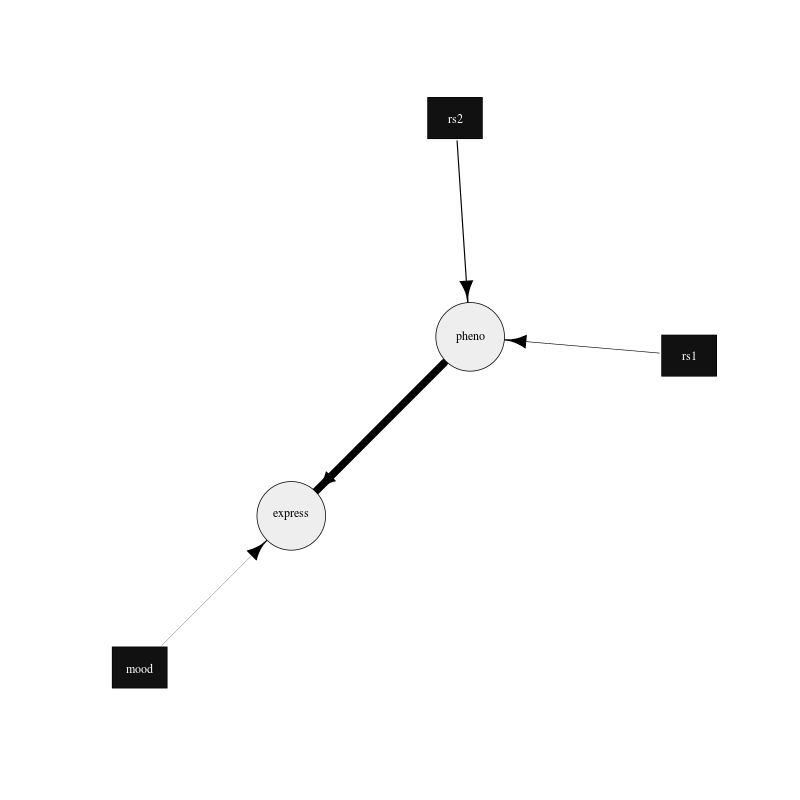
\includegraphics[width=400pt]{exampleGraph.png}}
\caption{Plot of the example network drawn using the igraph R package.}
\label{plot1-fig}
\end{center}}
\end{figure}
}

The edges are drawn proportional to the log likelihood difference between networks with and without the edge in question. The minimum and maximum thickness of the plotted edges can be changed by modifying the \code{minWidth} and \code{maxWidth} variables in the R file. The plot can easily be updated to your needs by following the igraphR package documentation. 

If a search is performed to find the best network (see parameter file \code{paras-plot-network2.txt}), it can be plotted as above and gives the following network: 
{\begin{figure}[ht]
{\begin{center}
{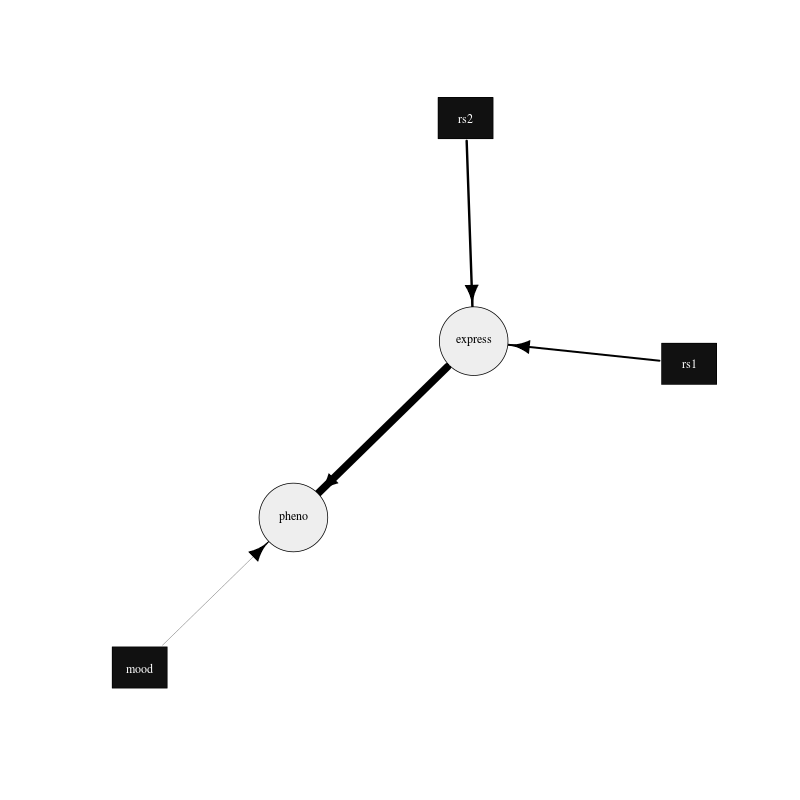
\includegraphics[width=400pt]{exampleGraph2.png}}
\caption{Plot of the best fit network drawn using the igraph R package.}
\label{plot2-fig}
\end{center}}
\end{figure}
}

%============ End of subsection "igraph-example"============


%================== End of section "plot-network"==================

\bibliographystyle{genepi}
\bibliography{/home/nrajh/work-other/tex/biblio}
\end{document}